\documentclass[a4paper, portrait,11pt]{article}
\usepackage{polski}
\usepackage[utf8]{inputenc}
\usepackage{amsmath}
\usepackage{graphicx}
\usepackage{hyperref}
\usepackage{listings}
\usepackage{subcaption}
\usepackage{numprint}
\usepackage{siunitx}
\usepackage[justification=centering]{caption}
\usepackage[margin=0.5in]{geometry}
\npdecimalsign{.}
\nprounddigits{3}

\title{\textbf{Zadanie 3 - Inteligentna Analiza Danych}}
\author{
  Adam Zambrzycki\\
  \texttt{Nr indeksu: 216933}
  \and
  Konrad Stępniak\\
  \texttt{Nr indeksu: 216892}
}

\begin{document}
\maketitle
  \begin{tabular}{ll}
    \textbf{Kierunek} & Informatyka\\
    \textbf{Rok akademicki} & {2018/19} \\
    \textbf{Semestr} & {4} \\
    \textbf{Grupa dziekańska}& {2} \\ \\ \\
  \end{tabular}

Symbol $\alpha$ będzie oznaczał współczynnik nauki, a $K$ liczbę centrów.
Współczynnik skalujący w sieci będzie nazywany sigmą.

\section{Osobna nauka warstw - Aproksymacja}
Do nauki wykorzystano następujące parametry: $\alpha=0.05$, liczba iteracji $= 20000$.
Optymalną sigmę uzyskano ze wzoru:
\begin{equation}
  \sigma = \frac{d}{\sqrt{2M}}
\end{equation}
Gdzie $d$ - maksymalna odległość między centrami, a $M$ to liczba centrów.
\subsection{Podzadanie 1}

\begin{figure}[!htb]
  \begin{minipage}{0.33\textwidth}
    \centering
    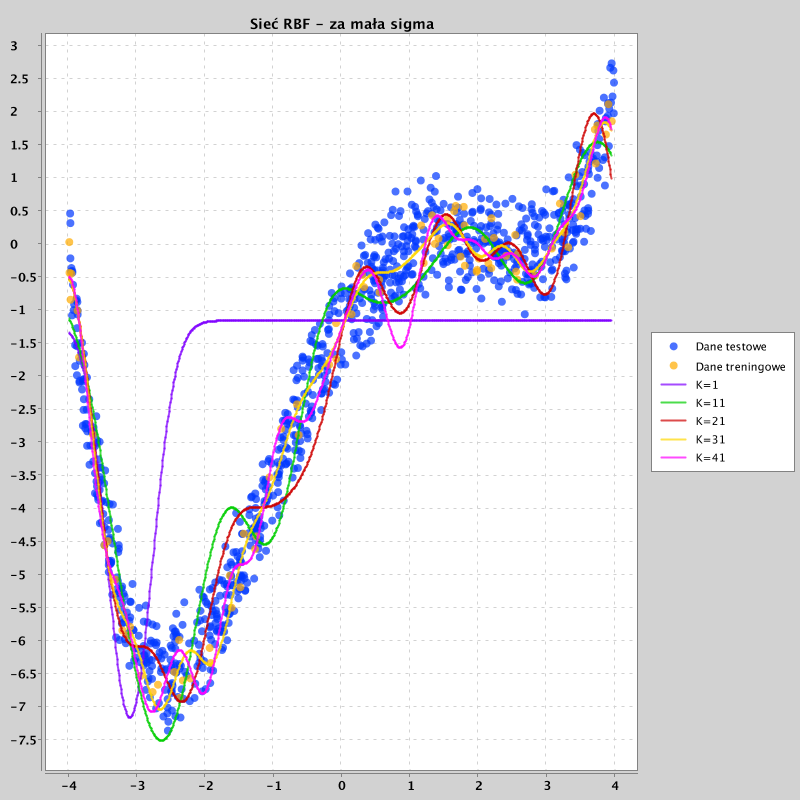
\includegraphics[width=1\linewidth]{../data/approximation3/1/small.png}
    \caption{\label{fig:1small}Za mała sigma}
  \end{minipage}
  \begin{minipage}{0.33\textwidth}
    \centering
    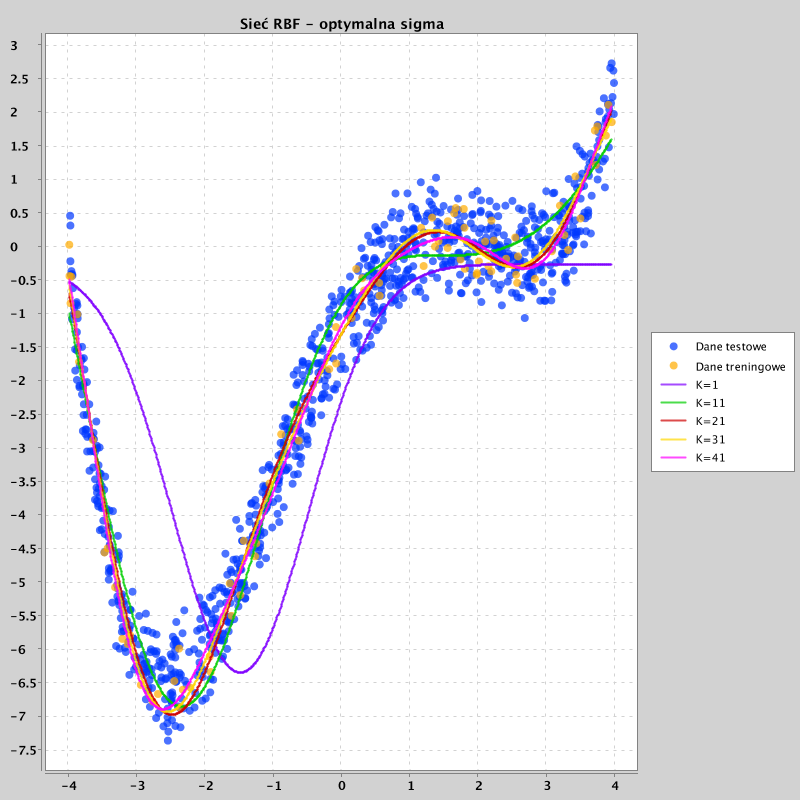
\includegraphics[width=1\linewidth]{../data/approximation3/1/optimal.png}
    \caption{\label{fig:1optimal}Optymalna sigma}
  \end{minipage}
  \begin{minipage}{0.33\textwidth}
    \centering
    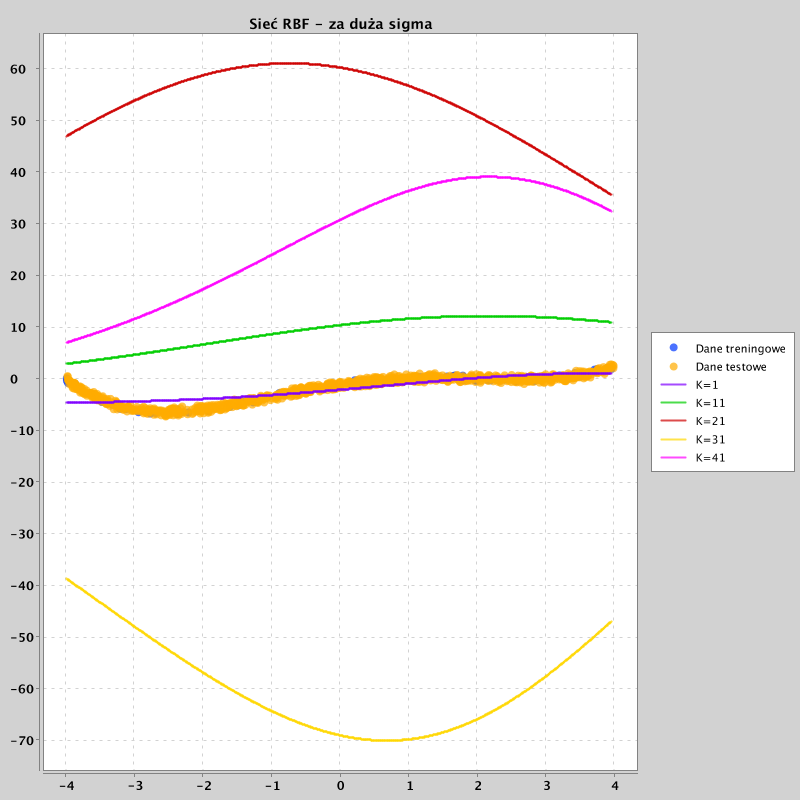
\includegraphics[width=1\linewidth]{../data/approximation3/1/big.png}
    \caption{\label{fig:1big}Za duża sigma}
  \end{minipage}\hfill
\end{figure}
Dla liczby $K >= 11$, gdy współczynnik skalujący 
jest zbyt mały sieć przybliża dane treningowe do pewnego stopnia, 
jednak tworzy pewne zakłócenia, co daje niedokładne przybliżenie.
Z drugiej strony, gdy sigma jest zbyt duża sieć praktycznie wcale nie aproksymuje danych jedynie je przecina w pewien sposób.
Sieć o $K=1$ daje takie same wyniki, jak $K=41$.
Gdy sigma jest optymalna, sieć o każdej liczbie neuronów oprócz $K=1$, aproksymuje tak samo dokładnie.

\subsection{Podzadanie 2}

Czerwone linie reprezentują funkcje pojedynczych neuronów.
\begin{figure}[!htb]
  \begin{minipage}{0.33\textwidth}
    \centering
    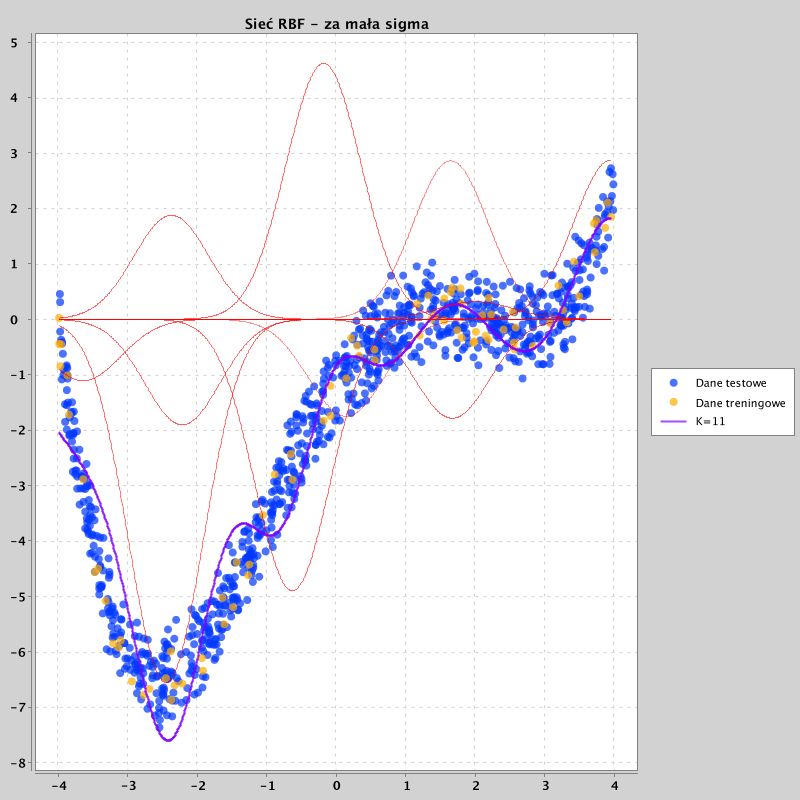
\includegraphics[width=1\linewidth]{../data/approximation3/2/small.png}
    \caption{\label{fig:2small}Za mała sigma}
  \end{minipage}
  \begin{minipage}{0.33\textwidth}
    \centering
    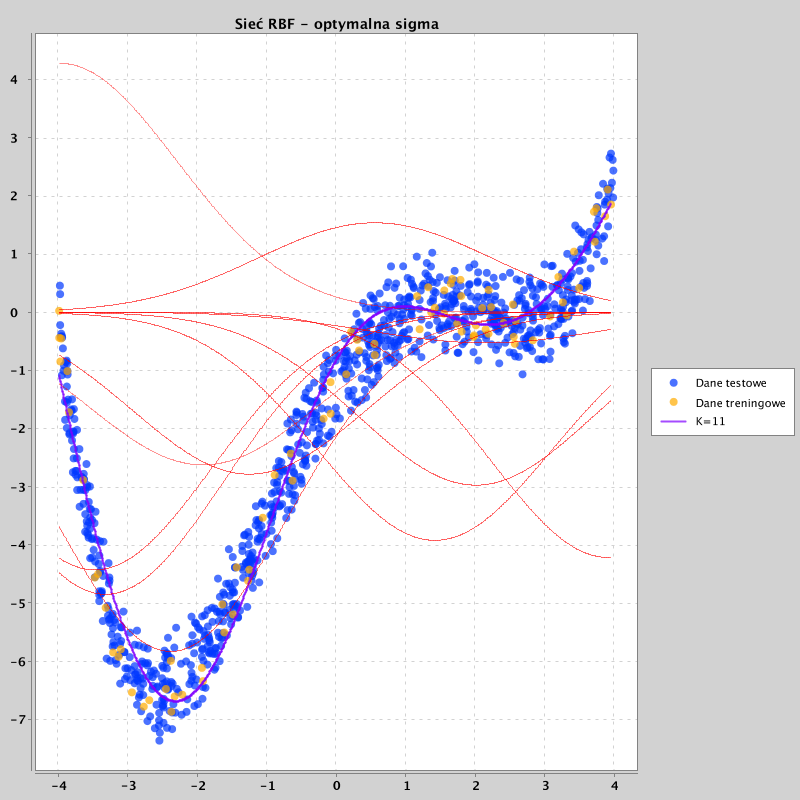
\includegraphics[width=1\linewidth]{../data/approximation3/2/optimal.png}
    \caption{\label{fig:2optimal}Optymalna sigma}
  \end{minipage}
  \begin{minipage}{0.33\textwidth}
    \centering
    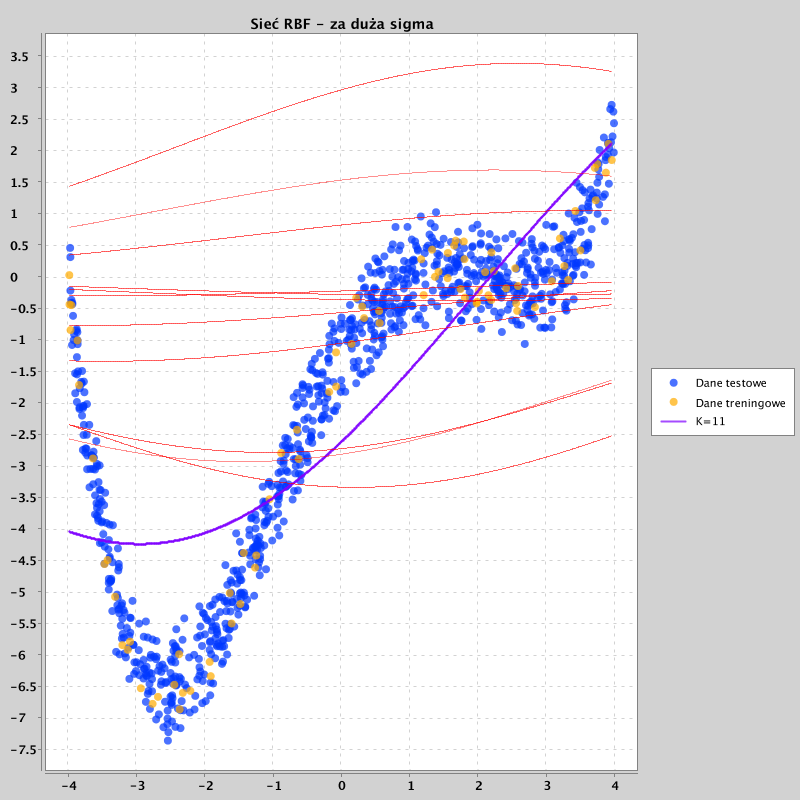
\includegraphics[width=1\linewidth]{../data/approximation3/2/big.png}
    \caption{\label{fig:2big}Za duża sigma}
  \end{minipage}\hfill
\end{figure}
Na podstawie poprzednich wyników wybrano $K=11$. Na Rysunku \ref{fig:2small} widać powód zakłóceń wykrytych na Rysunku \ref{fig:1small}.
Gdy sigma jest za mała funkcje aktywacji neuronów mają zbyt wąski obszar aktywacji.
Z drugiej strony na Rysunku \ref{fig:2big} widać, że przy dużym współczynniku skalującym funkcje neuronów są prawie stałe.
Nie da się stworzyć z kombinacji funkcji stałych dowolnej funkcji.
Jeśli zaś dobierzemy sigmę optymalnie, neurony będą realizowały funkcje nie za wąską i nie ze szeroką, co umożliwi bardzo dokładną aproksymację jak na Rysunku \ref{fig:2optimal}.


\subsection{Podzadanie 3}
Symbole $\epsilon_a$, $\epsilon_b$ oznaczają błędy średniokwadratowe odpowiednio dla zbioru treningowego i testowego. 
Symbol $\sigma$ w Tabeli \ref{table:approx3} oznacza odchylenie standardowe.
\begin{table}[h!]
  \caption{\label{table:approx3}Błąd średniokwadratowy oraz odchylenie dla zbioru treningowego i testowego dla 100 prób nauki}
  \centering
  \begin{tabular}{|l|n{1}{3}|n{1}{3}|n{1}{3}|n{1}{3}|}
    \hline
    \textbf{K} & \textbf{$avg(\epsilon_a)$} & \textbf{$\sigma(\epsilon_a)$} & \textbf{$avg(\epsilon_b)$} & \textbf{$\sigma(\epsilon_b)$}\\
    \hline
    1 & 2.2487527537653222 & 0.6261100919193574 & 1.955473836265807 & 0.5621825986540743 \\
    6 & 0.28568563944924996 & 0.2858213621279681 & 0.2522575453670399 & 0.19566409363294007 \\
    11 & 0.15128659994761162 & 0.11688975023198557 & 0.1680474127628648 & 0.07502859293396406 \\
    16 & 0.07765026065094292 & 0.02498215607290317 & 0.11514668896463105 & 0.01780284915773643 \\
    21 & 0.06057939963788164 & 0.016323733595582136 & 0.10661257959927159 & 0.009578394200630884 \\
    26 & 0.05789604352158822 & 0.009466525235758683 & 0.10751656209053062 & 0.007975489839156847 \\
    31 & 0.0515018661618608 & 0.005740971340396712 & 0.10206851520703669 & 0.005089507447365943 \\
    36 & 0.04704336994595712 & 0.0033461785075818125 & 0.09778242471482931 & 0.0032371893229406067 \\
    41 & 0.04561073842684816 & 0.0031295651169926855 & 0.09715678881154301 & 0.003091645909513203 \\
    \hline
  \end{tabular}
\end{table}
Losowy wybór centrów neuronów wprowadza dodatkowy błąd do sieci, 
gdyż przy małej ich liczbie mogą one zostać rozłożone nierównomiernie po całym zbiorze.
Wynika stąd bardzo duże odchylenie standardowe dla $K=1,6,11$.
Gdy $K=11$, błąd jest już relatywnie mały jednak nauka jest niestabilna, przez wspomniane losowanie centrów.
Zauważmy, że dla $K=16$, błąd zmniejsza się już dwukrotnie, a odchylenie standardowe jest bardzo małe.
Taka liczba neuronów zapewnia już reprezentatywność danych treningowych.
Przy $K=26,31,36,41$ średni błąd i odchylenie zmienia się nieznacząco w stosunku do $K=16$.
Za duża liczba neuronów nie zwiększa znacząco możliwości aproksymacyjnych sieci.
Błąd i odchylenie na zbiorze testowym zawsze jest większe niż na zbiorze treningowym.

\subsection{Podzadanie 4}
\begin{figure}[!htb]
  \centering
  \begin{minipage}{0.5\textwidth}
    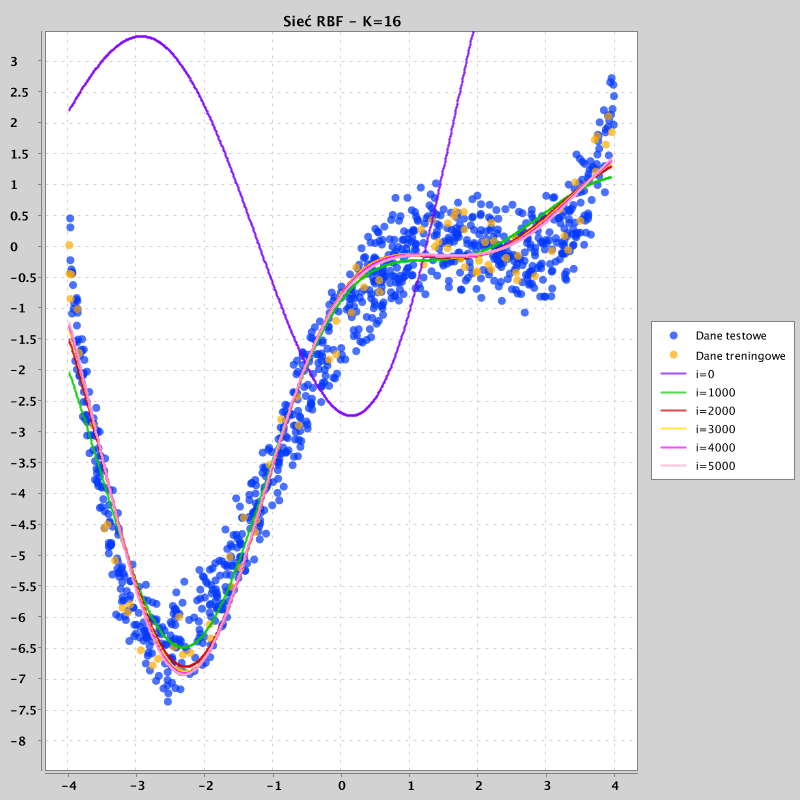
\includegraphics[width=1\linewidth]{../data/approximation3/4/chart.png}
    \caption{\label{fig:4chart}Zmiana funkcji sieci w różnych momentach}
  \end{minipage}\hfill
\end{figure}

Na podstawie obserwacji z Tabeli \ref{table:approx3},
Rysunek \ref{fig:4chart} został wygenerowany z parametrami $K=16$, liczba iteracji $= 5000$.
Można na nim wyraźnie zaobserwować, że już po $2000$ iteracji funkcja realizowana przez sieć wyglądała tak samo jak dla $i=5000$.
Gdy błąd przestanie się znacząco zmniejszać należy przestać uczyć sieć, gdyż nie da to lepszych efektów.

\subsection{Podsumowanie}
\begin{itemize}
  \item Błąd średniokwadratowy z każdą iteracją spada dosyć szybko, jednak w pewnym momencie osiąga próg, po którym dalsze uczenie sieci nie daje znaczących efektów.
  \item Potrzebna liczba neuronów w warstwie radialnej jest zależna od charakterystyki danych jakie aproksymujemy. Za mała nie przybliży jej wcale, a za duża daje prawie takie same wyniki jak optymalna, którą należy dobrać eksperymentalnie.
  \item Sieć można uznać za nauczoną, gdy jej błąd przestanie znacząco maleć. Zależy to od charakterystyki danych. Jest to dosyć ważny aspekt, gdyż wtedy można trenować sieć np. przy 5000 iteracjach, a nie 20000 iteracji, co zabiera czas i moc obliczeniową.
  \item Jeśli centra zostaną źle wylosowane to błąd znacząco się zwiększa, dlatego należy wybierać taką ich liczbe aby minimalizować błąd stworzony przez losowanie.
  \item Współczynnik skalujący ma ogromny wpływ na funkcje realizowaną przez sieć, gdy dobierzemy go źle to przy za małej wartości sieć będzie niedokładna. Przy za dużym współczynniku nie będzie aproksymowała wcale. Należy go dobierać tak, aby był optymalny.
\end{itemize}

\section{Osobna nauka warstw - klasyfikacja}
Wykorzystano parametry nauki: $\alpha=0.05$, optymalna sigma, liczba iteracji $=5000$.
Centra dobierano za pomocą algorytmu K-Średnich.
\subsection{Podzadanie 1}
\begin{figure}[!htb]
  \begin{minipage}{0.33\textwidth}
    \centering
    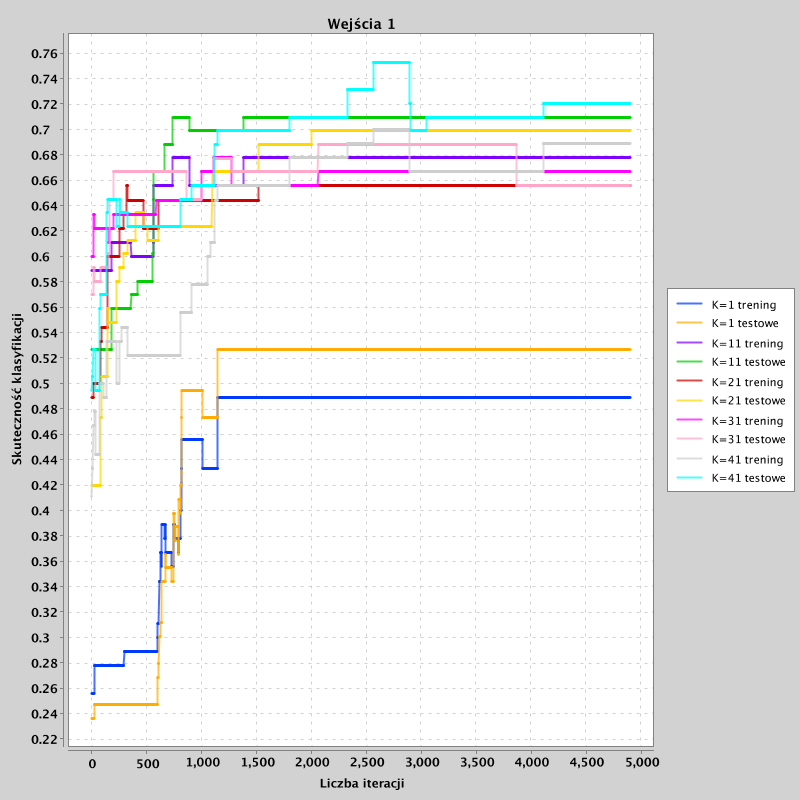
\includegraphics[width=1\linewidth]{../data/classification4/1/1_1.png}
    \caption{\label{fig:41_1_1}}
  \end{minipage}
  \begin{minipage}{0.33\textwidth}
    \centering
    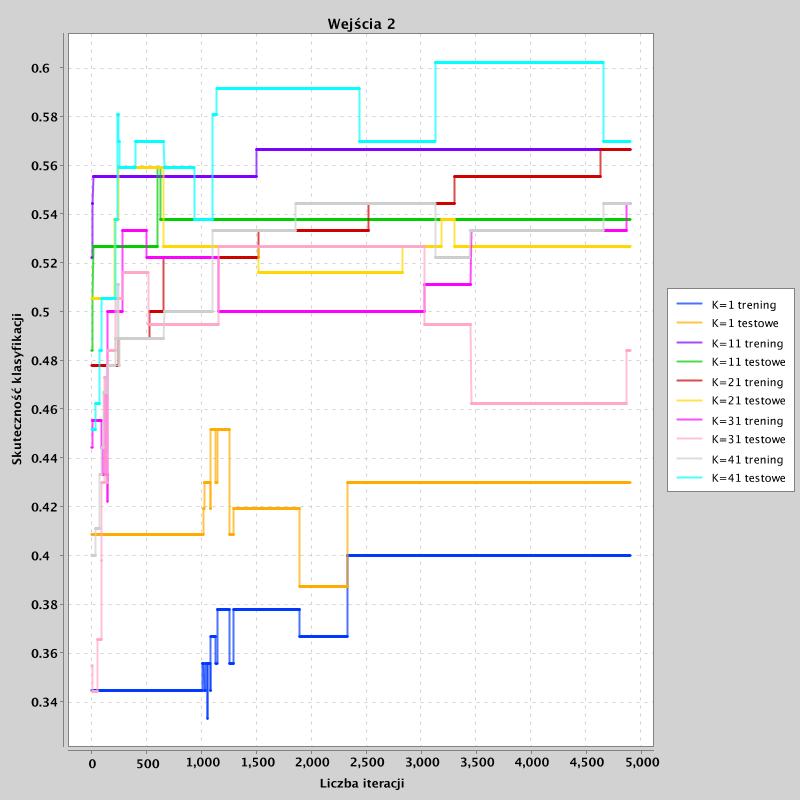
\includegraphics[width=1\linewidth]{../data/classification4/1/1_2.png}
    \caption{\label{fig:41_1_2}}
  \end{minipage}
  \begin{minipage}{0.33\textwidth}
    \centering
    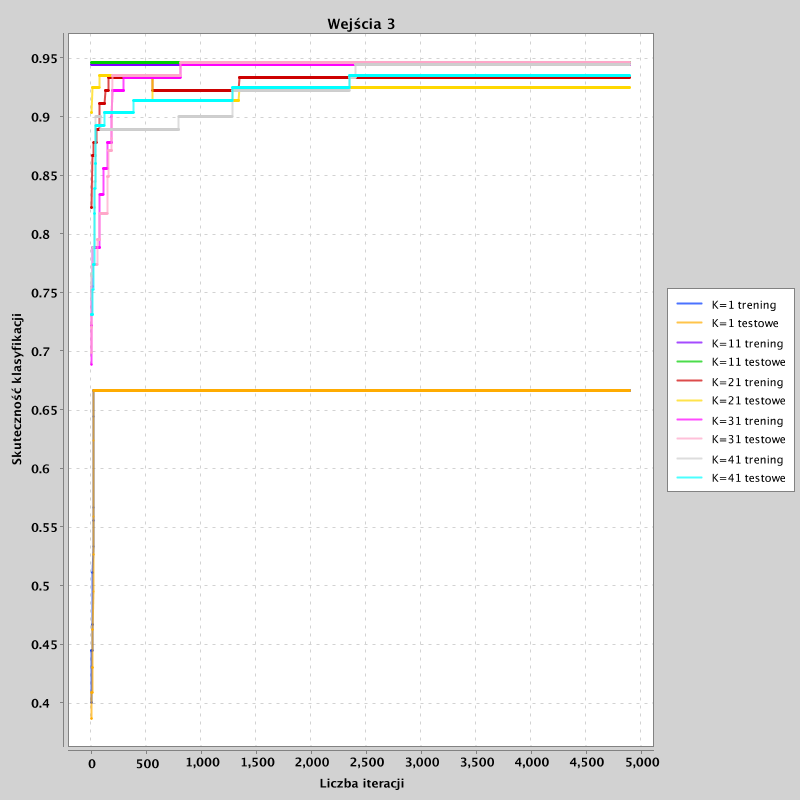
\includegraphics[width=1\linewidth]{../data/classification4/1/1_3.png}
    \caption{\label{fig:41_1_3}}
  \end{minipage}\hfill
\end{figure}

Dla cech (wejść) 1,2 przedstawionych na Rysunkach \ref{fig:41_1_1}, \ref{fig:41_1_2}, 
skuteczność klasyfikacji stosunkowo niska - 60-70\% niezależnie od $K$. 
Nie są one reprezentatywne. Z drugiej strony dla cech 3,4 na Rysunkach \ref{fig:41_1_3}, \ref{fig:41_1_4}
skutecnzość sięga 95\% dla $K >= 11$. Większa liczba neuronów niż $11$ nie zwiększa skuteczności.
Na podstawie jednej wybranej cechy z czterech można dokonać bardzo dobrej klasyfikacji.

Na Rysunku \ref{fig:41_2_1,2} widać, że po połączeniu 2 słabo reprezentatywnych cech,
można zwiększyć zdolności sieci o około 15\%. Jednak kombinacja dwóch najbardziej charakterystycznych cech 
na Rysunku \ref{fig:41_2_3,4} jest skuteczniejsza o tylko 1\%. 

Kombinacje 3 wejść na rysunkach \ref{fig:41_3_1,2,3} - \ref{fig:41_3_2,3,4} oraz 4 wejść na Rysunku \ref{fig:41_4_1,2,3,4} 
również nie polepszają klasyfikacji.

Skuteczność dla każdej z możliwych kombinacji rośnie skokowo. Jeśli cecha nie jest charakterystyczna to czasami nawet spada jak na Rysunku \ref{fig:41_1_2}.
Po około 3000 iteracji przestaje rosnąć i zatrzymuje się w miejscu.

\begin{figure}[!htb]
  \begin{minipage}{0.33\textwidth}
    \centering
    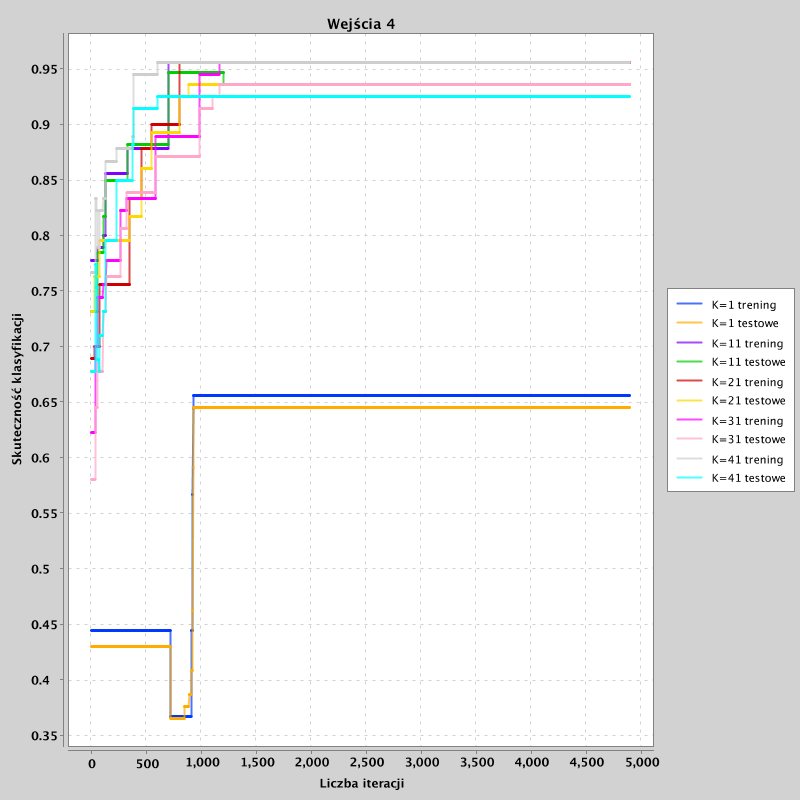
\includegraphics[width=1\linewidth]{../data/classification4/1/1_4.png}
    \caption{\label{fig:41_1_4}}
  \end{minipage}
  \begin{minipage}{0.33\textwidth}
    \centering
    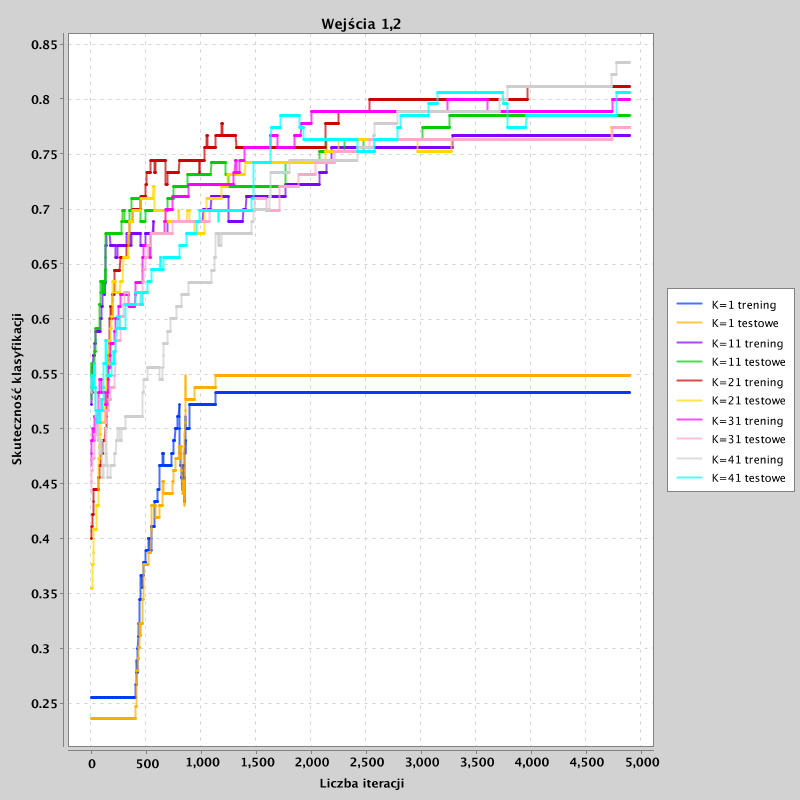
\includegraphics[width=1\linewidth]{../data/classification4/1/2_1,2.png}
    \caption{\label{fig:41_2_1,2}}
  \end{minipage}
  \begin{minipage}{0.33\textwidth}
    \centering
    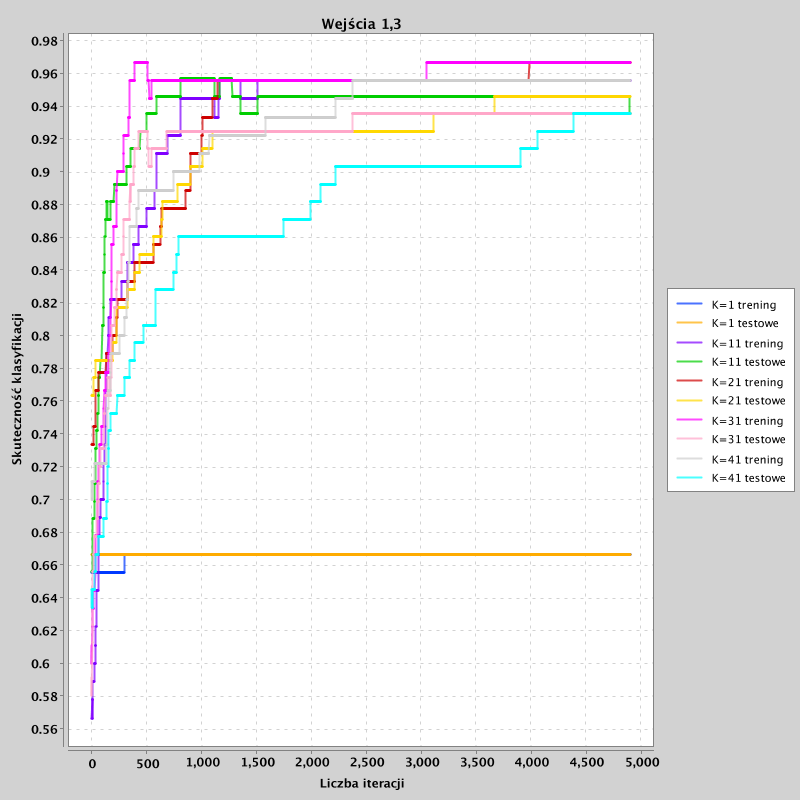
\includegraphics[width=1\linewidth]{../data/classification4/1/2_1,3.png}
    \caption{\label{fig:41_2_1,3}}
  \end{minipage}\hfill
\end{figure}
\begin{figure}[!htb]
  \begin{minipage}{0.33\textwidth}
    \centering
    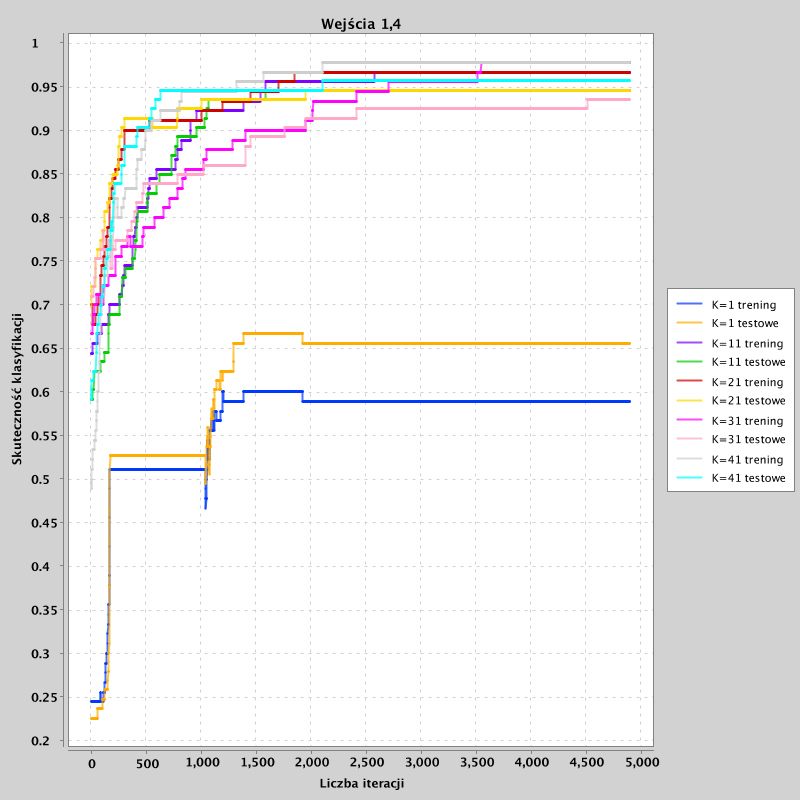
\includegraphics[width=1\linewidth]{../data/classification4/1/2_1,4.png}
    \caption{\label{fig:41_2_1,4}}
  \end{minipage}
  \begin{minipage}{0.33\textwidth}
    \centering
    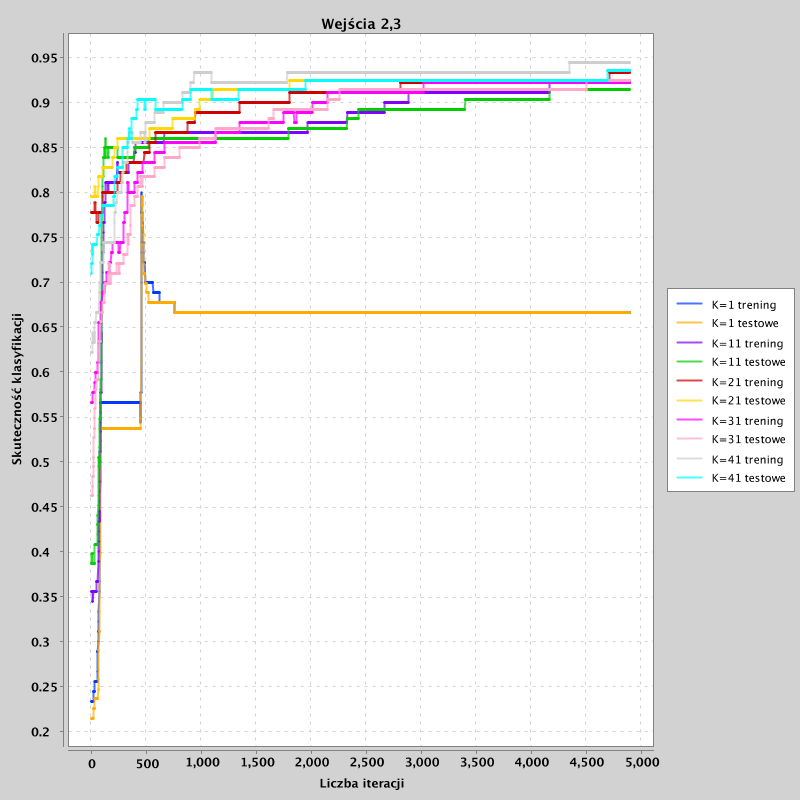
\includegraphics[width=1\linewidth]{../data/classification4/1/2_2,3.png}
    \caption{\label{fig:41_2_2,3}}
  \end{minipage}
  \begin{minipage}{0.33\textwidth}
    \centering
    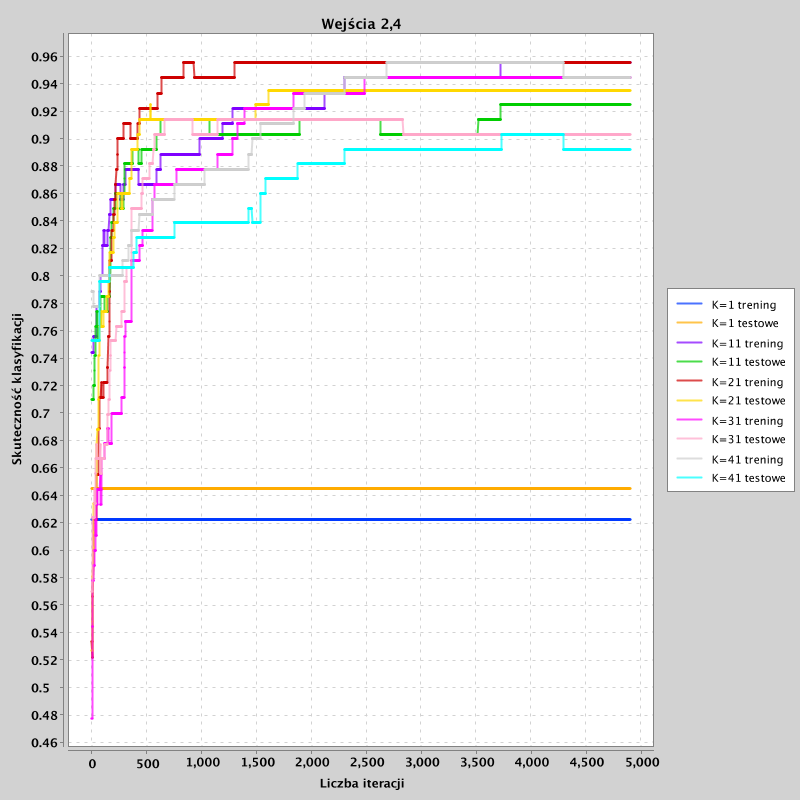
\includegraphics[width=1\linewidth]{../data/classification4/1/2_2,4.png}
    \caption{\label{fig:41_2_2,4}}
  \end{minipage}\hfill
\end{figure}
\begin{figure}[!htb]
  \begin{minipage}{0.33\textwidth}
    \centering
    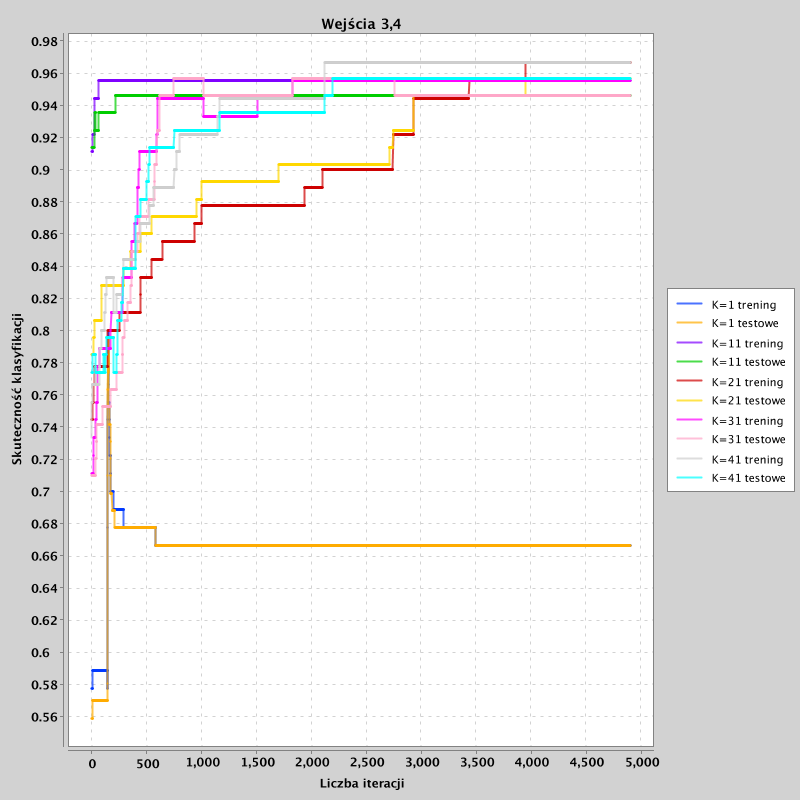
\includegraphics[width=1\linewidth]{../data/classification4/1/2_3,4.png}
    \caption{\label{fig:41_2_3,4}}
  \end{minipage}
  \begin{minipage}{0.33\textwidth}
    \centering
    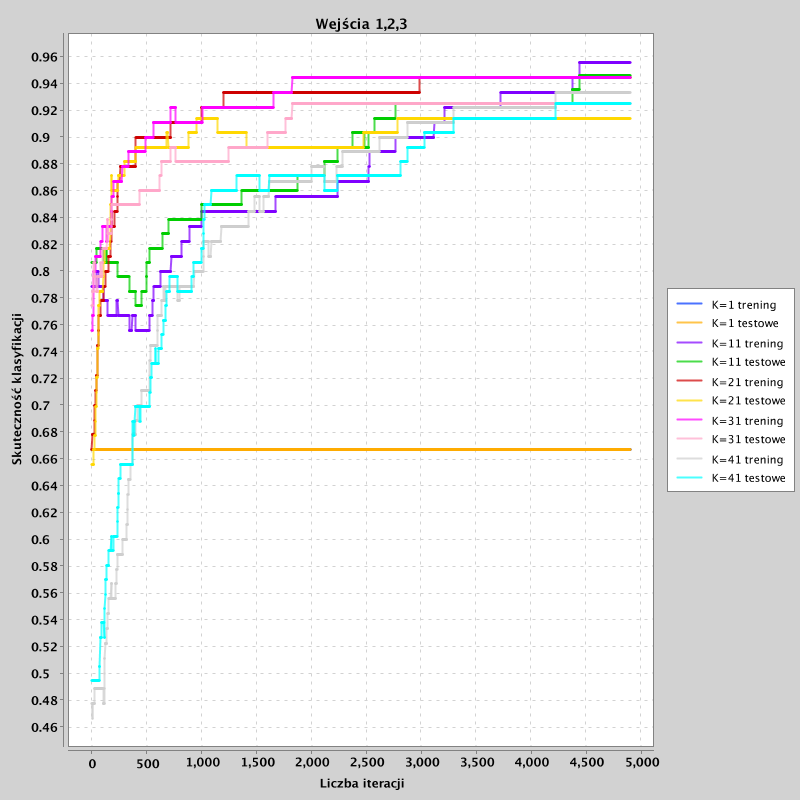
\includegraphics[width=1\linewidth]{../data/classification4/1/3_1,2,3.png}
    \caption{\label{fig:41_3_1,2,3}}
  \end{minipage}
  \begin{minipage}{0.33\textwidth}
    \centering
    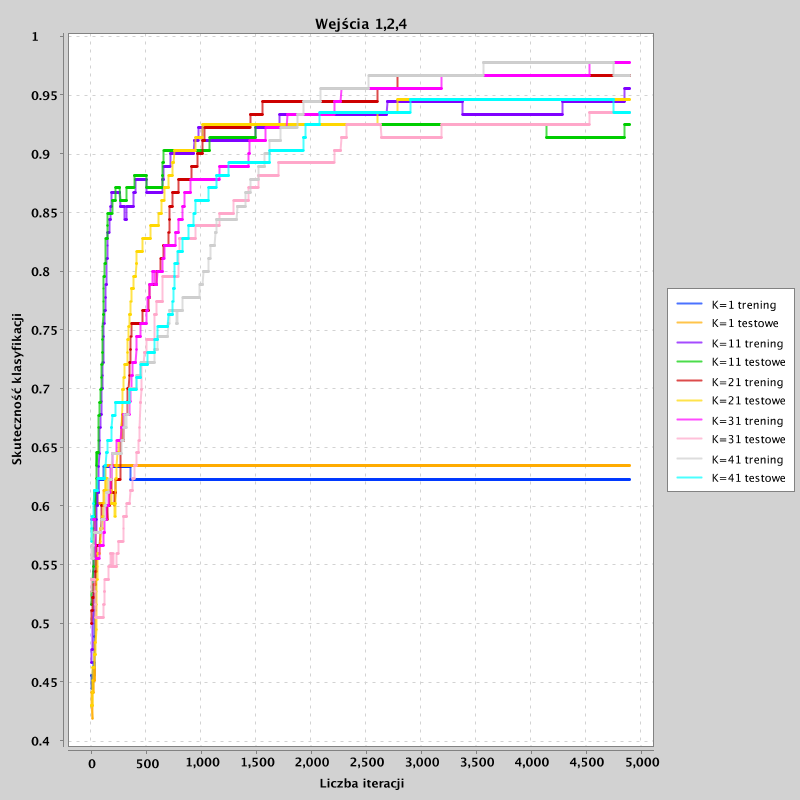
\includegraphics[width=1\linewidth]{../data/classification4/1/3_1,2,4.png}
    \caption{\label{fig:41_3_1,2,4}}
  \end{minipage}\hfill
\end{figure}
\begin{figure}[!htb]
  \begin{minipage}{0.33\textwidth}
    \centering
    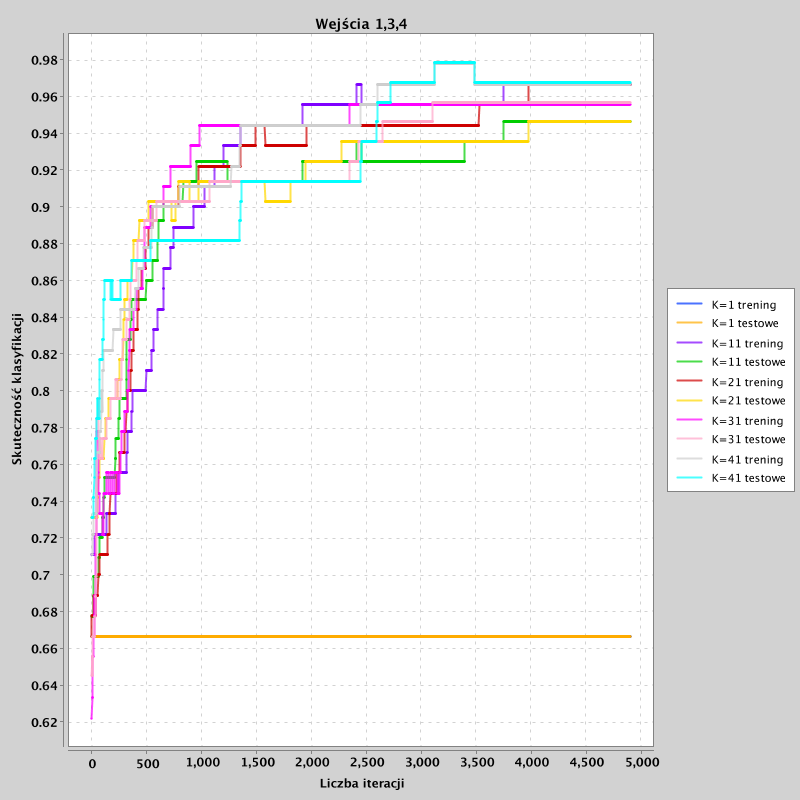
\includegraphics[width=1\linewidth]{../data/classification4/1/3_1,3,4.png}
    \caption{\label{fig:41_3_1,3,4}}
  \end{minipage}
  \begin{minipage}{0.33\textwidth}
    \centering
    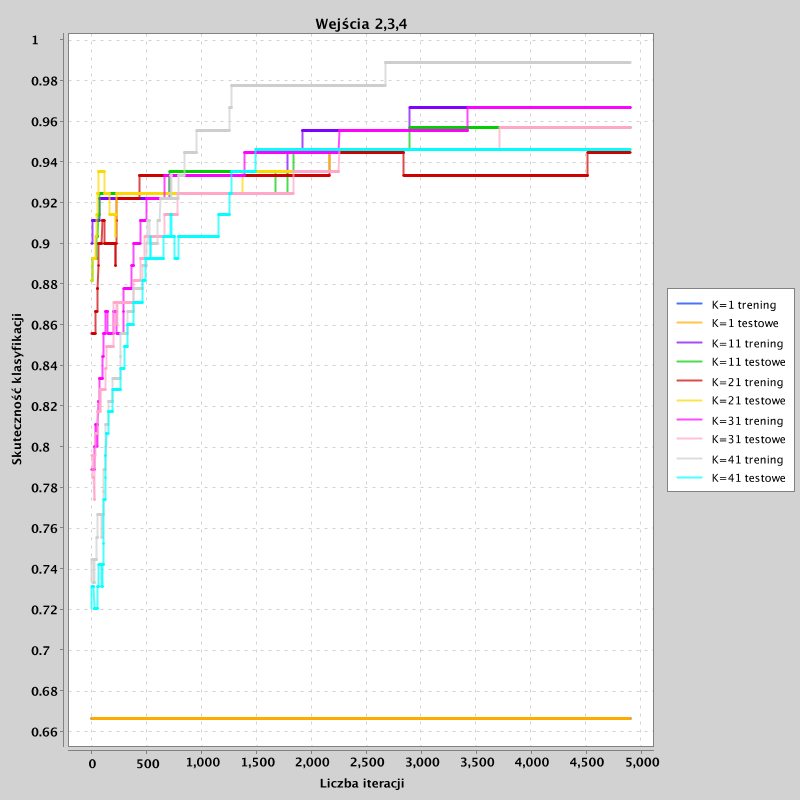
\includegraphics[width=1\linewidth]{../data/classification4/1/3_2,3,4.png}
    \caption{\label{fig:41_3_2,3,4}}
  \end{minipage}
  \begin{minipage}{0.33\textwidth}
    \centering
    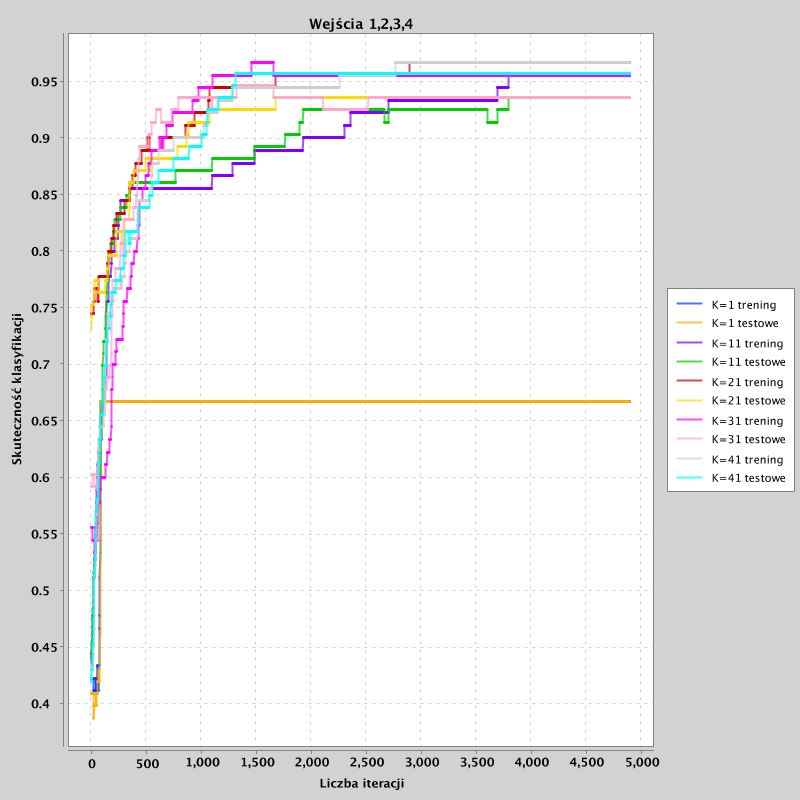
\includegraphics[width=1\linewidth]{../data/classification4/1/4_1,2,3,4.png}
    \caption{\label{fig:41_4_1,2,3,4}}
  \end{minipage}\hfill
\end{figure}

\nprounddigits{2}
\subsection{Podzadanie 2}
\begin{table}[h!]
  \caption{\label{table:classify4}Procent klasyfikacji oraz odchylenie dla zbioru treningowego i testowego dla 100 prób nauki}
  \centering
  \begin{tabular}{|l|n{1}{3}|n{1}{3}|n{1}{3}|n{1}{3}|}
    \hline
    \textbf{K} & \textbf{$avg(p_a)$} & \textbf{$\sigma(p_a)$} & \textbf{$avg(p_b)$} & \textbf{$\sigma(p_b)$} \\
    \hline
    1 & 0.6666666666666659 & 0 & 0.6666666666666659 & 0 \\
    6 & 0.935111111111111 & 0.0053794304164045135 & 0.928494623655913 & 0.009542064166289733 \\
    11 & 0.9368888888888887 & 0.005183068350973578 & 0.9307526881720424 & 0.01057049955048994 \\
    16 & 0.9371111111111108 & 0.006130272988503856 & 0.9308602150537629 & 0.01056338744688961 \\
    21 & 0.9378888888888883 & 0.006866450913546816 & 0.9324731182795698 & 0.01043398664146946 \\
    26 & 0.9398888888888883 & 0.0056862407030773094 & 0.9349462365591399 & 0.010129808430869264 \\
    31 & 0.9422222222222213 & 0.004444444444444427 & 0.9375268817204311 & 0.010051894484440608 \\
    36 & 0.9423333333333324 & 0.004358898943540653 & 0.9377419354838716 & 0.010676612602035777 \\
    41 & 0.9429999999999988 & 0.004622809791714378 & 0.9398924731182804 & 0.010869792434046578 \\
    \hline
  \end{tabular}
\end{table}
W Tabeli \ref{table:classify4} $p_a$, $p_b$ oznaczają odpowiednio procent klasyfikacji dla zbioru treningowego i testowego.
Procent poprawnie sklasyfikowanych obiektów  w zbiorze testowym jest zawsze taki sam, 
albo bardzo zbliżony do zbioru treningowego. 
Odchylenie standardowe na poziomie $0.01$ oznacza, że sieć jest bardzo stabilna i dla każdej próby daje takie samą skuteczność.
Dla $K >= 6$ skuteczność nie zmienia się, tyle neuronów wystarczy aby klasyfikować z dużą dokładnością.

\subsection{Podzadanie 3}
\begin{figure}[!htb]
  \begin{minipage}{0.33\textwidth}
    \centering
    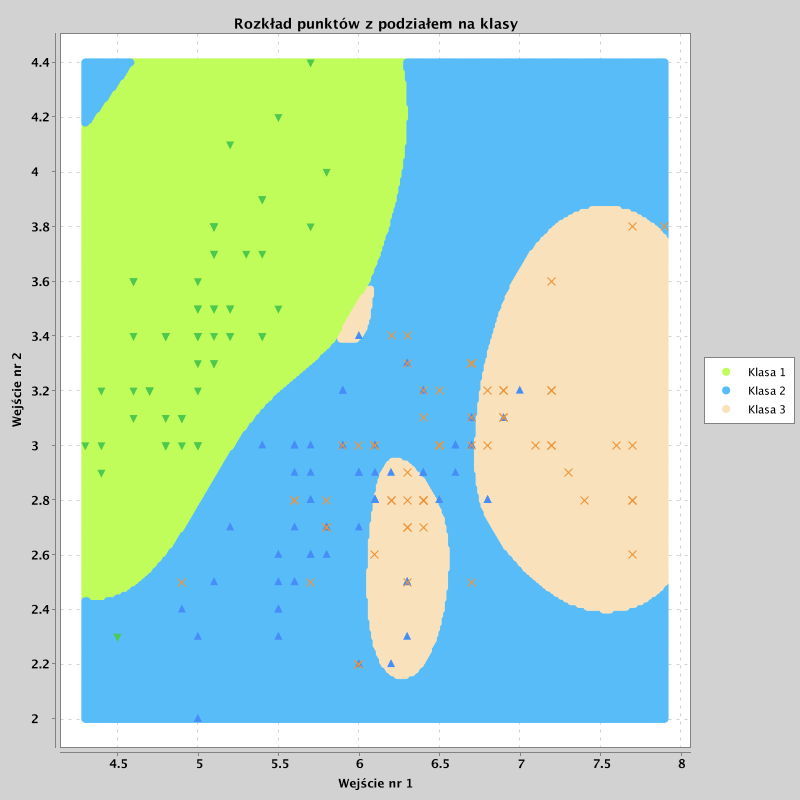
\includegraphics[width=1\linewidth]{../data/classification4/3/2_1,2.png}
    \caption{\label{fig:43_2_1,2}}
  \end{minipage}
  \begin{minipage}{0.33\textwidth}
    \centering
    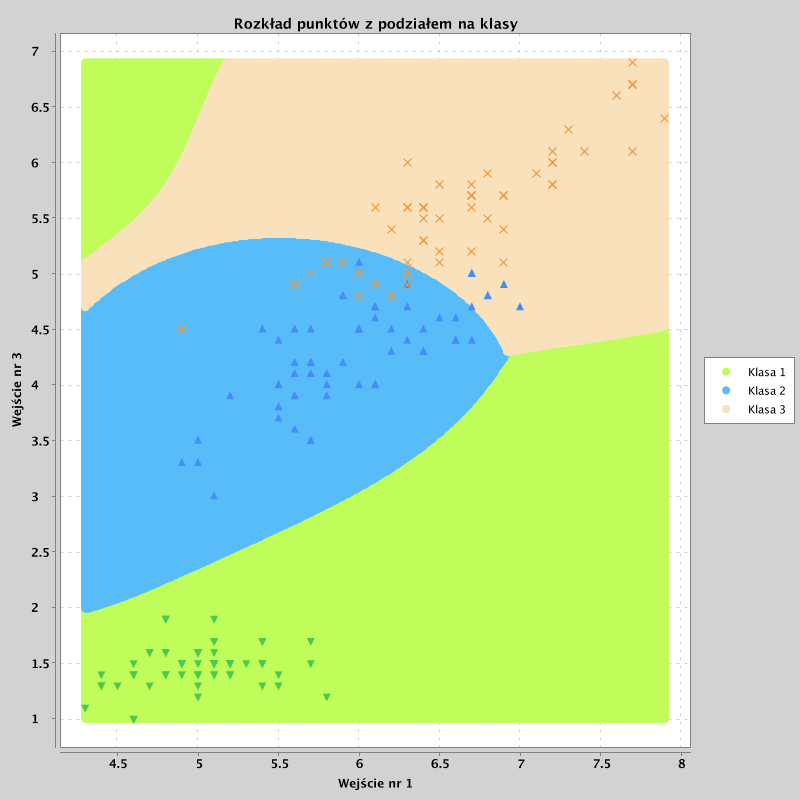
\includegraphics[width=1\linewidth]{../data/classification4/3/2_1,3.png}
    \caption{\label{fig:43_2_1,3}}
  \end{minipage}
  \begin{minipage}{0.33\textwidth}
    \centering
    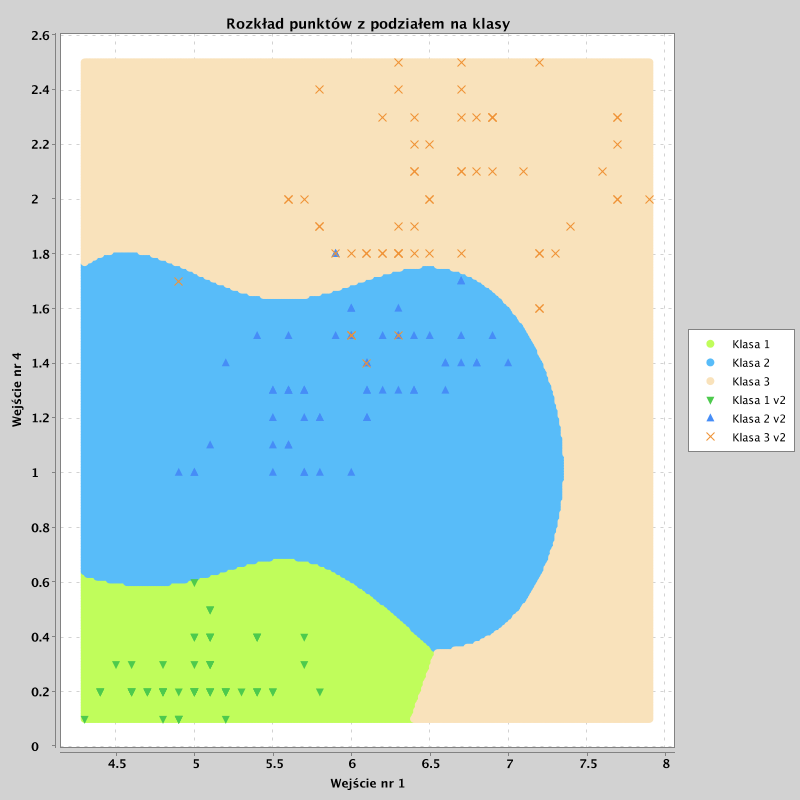
\includegraphics[width=1\linewidth]{../data/classification4/3/2_1,4.png}
    \caption{\label{fig:43_2_1,4}}
  \end{minipage}\hfill
\end{figure}
\begin{figure}[!htb]
  \begin{minipage}{0.33\textwidth}
    \centering
    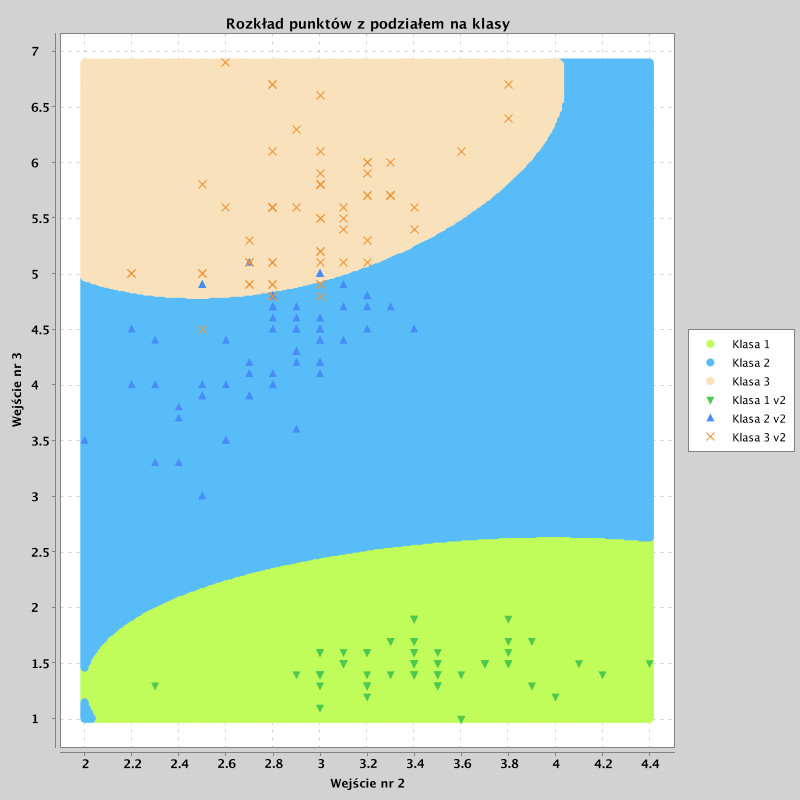
\includegraphics[width=1\linewidth]{../data/classification4/3/2_2,3.png}
    \caption{\label{fig:43_2_2,3}}
  \end{minipage}
  \begin{minipage}{0.33\textwidth}
    \centering
    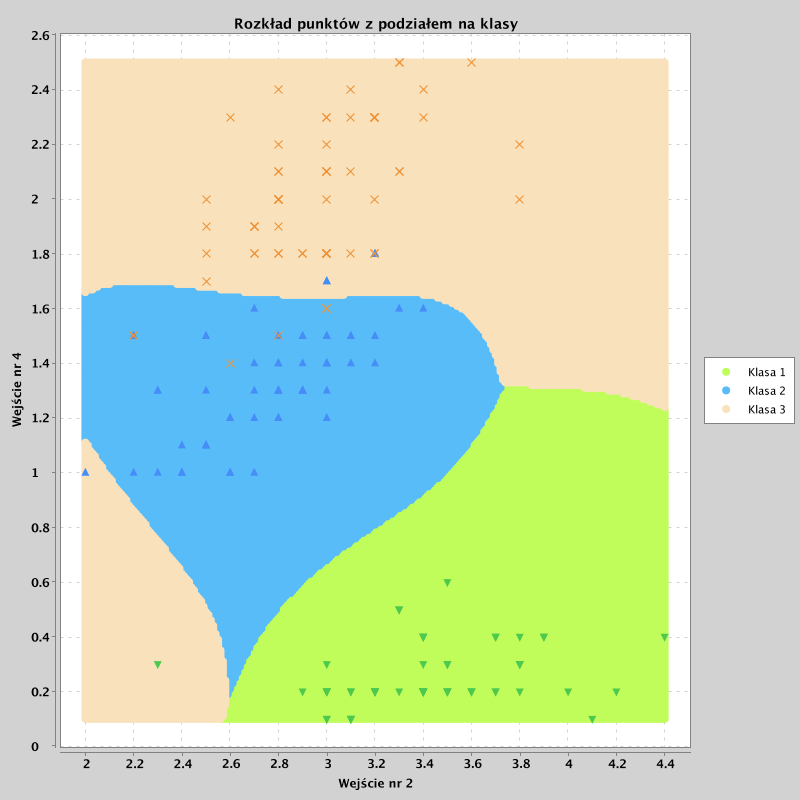
\includegraphics[width=1\linewidth]{../data/classification4/3/2_2,4.png}
    \caption{\label{fig:43_2_2,4}}
  \end{minipage}
  \begin{minipage}{0.33\textwidth}
    \centering
    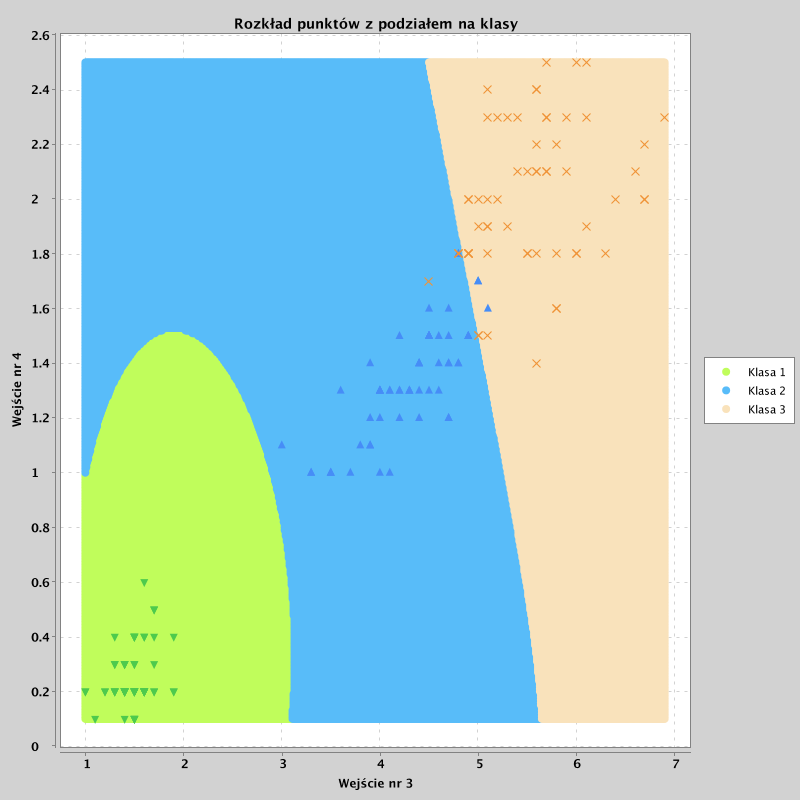
\includegraphics[width=1\linewidth]{../data/classification4/3/2_3,4.png}
    \caption{\label{fig:43_2_3,4}}
  \end{minipage}\hfill
\end{figure}

Rysunki zostały wygenerowane dla $K=6$. Zaokrąglone obszary wyznaczane na Rysunkach \ref{fig:43_2_1,2} - \ref{fig:43_2_3,4}
przypominają kształtem funkcję gaussowską neuronów radialnych.
Na granicach obszarów decyzyjnych zachodzą niejednoznaczności w klasyfikacji.
Po redukcji, gdy współrzędne w odpowiednich osiach mają taką samą wartość nie ma sposobu na odróżnienie obiektów.

\subsection{Podsumowanie}
\begin{itemize}
  \item Skuteczność sieci zmienia się skokowo, jest bardzo zbliżona na zbiorze treningowym i testowym.
  \item Większa liczba neuronów nie oznacza zwiększenia skuteczności klasyfikacji. Optymalna liczba zależy od charakterystyki zbioru.
  \item Redukcja wektora wejściowego do różnych kombinacji współrzędnych może wyłonić współrzędne reprezentatywne. Dzięki czemu będzie można rozpoznać obiekty po 1 z cech.
  \item Gdy znajdziemy jedną cechę charakterystyczną, dodanie większej ich liczby nie zwiększy znacząco skuteczności.
  \item Sieć po pewnej liczbie iteracji przestaje się uczyć - procent skuteczności przestaje rosnąć.
\end{itemize}
\section{Nauka obu warstw}
\newcommand{\partialSigma}{\frac{\partial}{\partial{\sigma_{k}}}}

\subsection{Wyprowadzenie wzorów}
\subsubsection{Pochodna po współczynniku skalującym}
\begin{align*}
  \frac{\partial E}{\partial{\sigma_{k}}}&= \frac{1}{2N} \sum_{j=1}^{N} (f(x^j) - y^j)^2\\
  &= \frac{1}{2N} \sum_{j=1}^{N} 2 (f(x^j) - y^j) f'(x^j)\\
  &= \frac{1}{N} \sum_{j=1}^{N} f(x^j - y^j) \partialSigma \sum_{k=0}^{K} w_k z_k(x^j)\\
  \partialSigma \sum_{k=0}^{K} w_k z_k(x^j) &= \sum_{k=0}^{K} w_k z_k(x^j) =  w_k \frac{\partial}{\partial{\sigma_{k}}}z_k(x^j)
\end{align*}
Ponieważ tylko $w_k \partialSigma z_k(x^j)$ zależy od $\sigma_k$, dla $k=0, ..., K$
\begin{align*}
  \frac{\partial}{\partial{\sigma_{k}}}z_k(x^j) &= \partialSigma exp(-d^2(x^j, c_k) \frac{1}{2\sigma_k^2})\\
  &= z_k(x^j) \partialSigma ( \frac{1}{2\sigma_k^2}) \\
  &= z_k(x^j) \frac{-1}{2} d^2(x^j, c_k) \partialSigma {\sigma_k^{-2}}\\
  &= z_k(x^j) \frac{-1}{2} d^2(x^j, c_k) -2 \sigma_k^{-3}\\
  &= z_k(x^j) d^2(x^j, c_k) \frac{1}{\sigma_k^3}
\end{align*}
Ostatecznie
\begin{equation}
  \frac{\partial E}{\partial{\sigma_{k}}} = \frac{1}{N} \sum_{j=1}^{N} f(x^j - y^j) z_k(x^j) w_k d^2(x^j, c_k) \frac{1}{\sigma_k^3}
\end{equation}
\subsubsection{Pochodna po koordynacie centrum neuronu}
Analogicznie jak w poprzednim wyprowadzeniu.
\begin{align*}
  \frac{\partial}{\partial{c_{k,i}}}z_k(x^j) &= \frac{\partial}{\partial{c_{k,i}}} exp(-d^2(x^j, c_k) \frac{1}{2\sigma_k^2})\\
    &= z_k(x^j) \frac{\partial}{\partial{c_{k,i}}} -d^2(x^j, c_k) \frac{1}{2\sigma_k^2}\\
    &= z_k(x^j) \frac{-1}{2\sigma_k^2} \frac{\partial}{\partial{c_{k,i}}} d^2(x^j, c_k) \\
  \frac{\partial}{\partial{c_{k,i}}} d^2(x^j, c_k) &= \frac{\partial}{\partial{c_{k,i}}} \sqrt{\sum_{i = 1}^{n} (x_i - c_{k,i})^2}^2\\
  &= \frac{\partial}{\partial{c_{k,i}}} \sum_{i = 1}^{n} (x_i - c_{k,i})^2\\
  &= \sum_{i = 1}^{n} 2 (x_i - c_{k,i}) (-1)\\
  &= -2 \sum_{i = 1}^{n} (x_i - c_{k,i})\\
  &= -2 (x_i - c_{k,i})
\end{align*}
Ponieważ tylko $x_i - c_{k,i}$ zależy od $c_{k,i}$.
\begin{align*}
  \frac{\partial}{\partial{c_{k,i}}} &= z_k(x^j) \frac{-1}{2\sigma_k^2} (-2) (x_i - c_{k,i})\\
  \frac{\partial}{\partial{c_{k,i}}} &= z_k(x^j) \frac{1}{\sigma_k^2} (x_i - c_{k,i})\\
\end{align*}
Ostateczny wzór:
\begin{equation}
\frac{\partial E}{\partial{c_{k,i}}} = \frac{1}{N} \sum_{j=1}^{N} f(x^j - y^j) w_k z_k(x^j) \frac{1}{\sigma_k^2} (x_i - c_{k,i})
\end{equation}
\subsection{Podpunkt 2}

\begin{figure}[!htb]
  \begin{minipage}{0.33\textwidth}
    \centering
    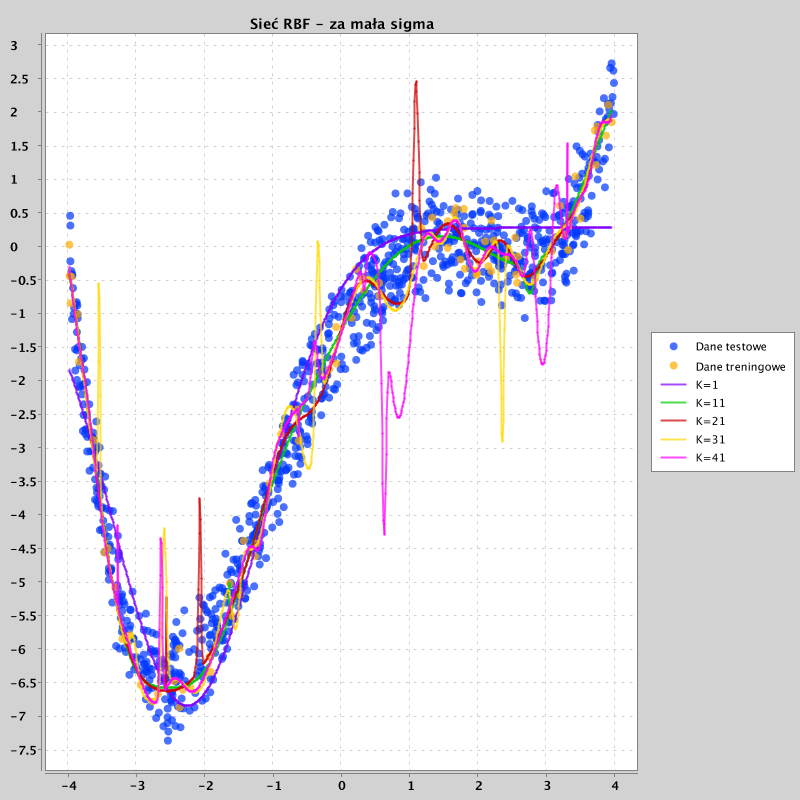
\includegraphics[width=1\linewidth]{../data/approximation3/1/derivatives/small.png}
    \caption{\label{fig:1smallderivative}Za mała sigma}
  \end{minipage}
  \begin{minipage}{0.33\textwidth}
    \centering
    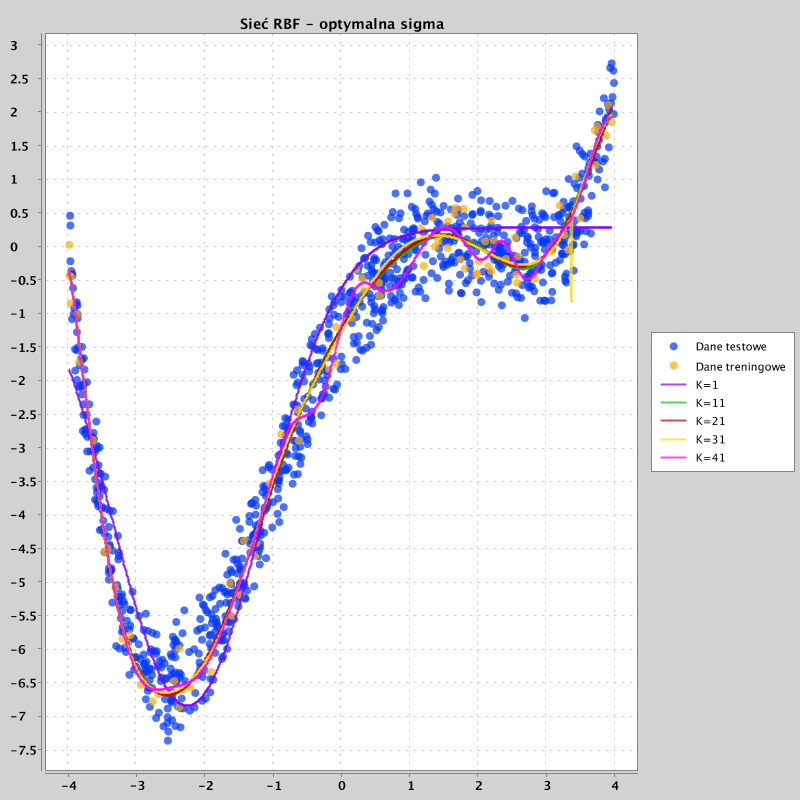
\includegraphics[width=1\linewidth]{../data/approximation3/1/derivatives/optimal.png}
    \caption{\label{fig:1optimalderivative}Optymalna sigma}
  \end{minipage}
  \begin{minipage}{0.33\textwidth}
    \centering
    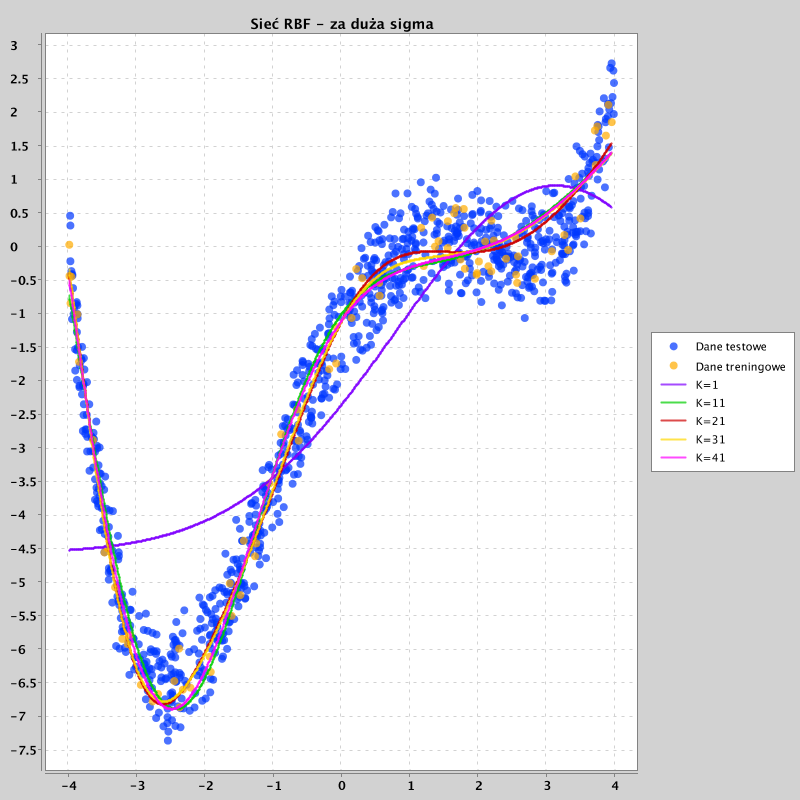
\includegraphics[width=1\linewidth]{../data/approximation3/1/derivatives/big.png}
    \caption{\label{fig:1bigderivative}Za duża sigma}
  \end{minipage}\hfill
\end{figure}

Na rysunkach \ref{fig:1smallderivative} - \ref{fig:1bigderivative} zaprezentowano uczenie obu wartsw dla różnej liczby neuronów i różnych sigm.
Ciekawym przypadkiem jest gdy K=1 dla za małej sigmy, udało się tak ustalić funkcję, że jest bardzo dobrze przybliża dane treningowe i testowe poza prawym końcem wykresu.
Jest to czysty przypadek, wynikający z rozłożenia danych.
W odróżnieniu od osobnej nauki warstw tutaj wybór nie ma aż tak dużego wpływu na nauke sieci. Sama się dopasowuje.
Jednak w przypadku za małej sigmy funkcja przy za dużej liczbie neuronów tworzy niepożądane zniekształcenia.
W przypadku za dużej sigmy, koniec funkcji jest nie do końca przybliżony. 
\begin{figure}[!htb]
  \begin{minipage}{0.33\textwidth}
    \centering
    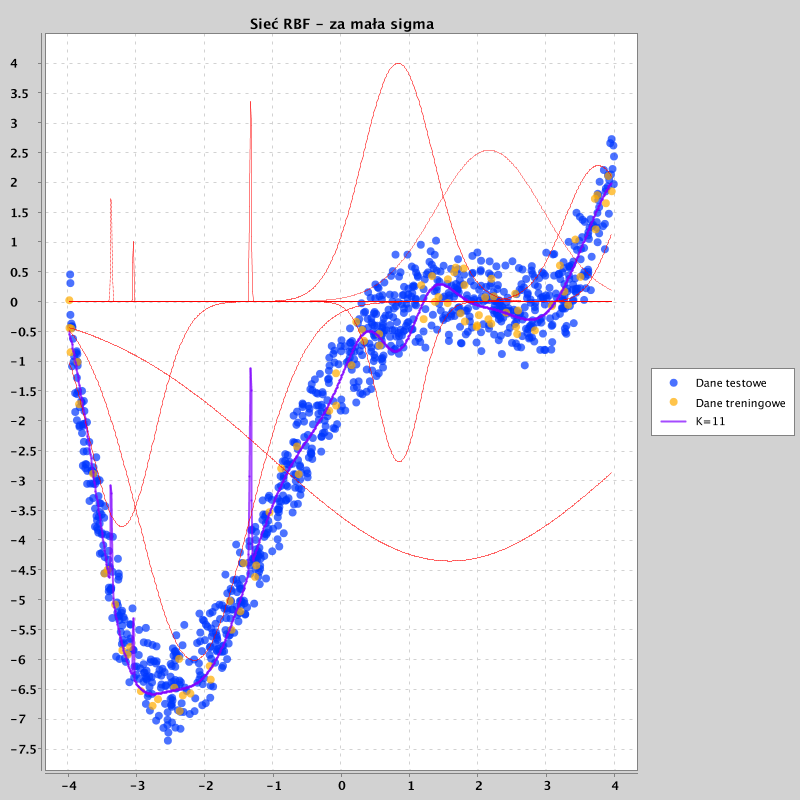
\includegraphics[width=1\linewidth]{../data/approximation3/2/derivatives/small.png}
    \caption{\label{fig:2smallderivative}Za mała sigma}
  \end{minipage}
  \begin{minipage}{0.33\textwidth}
    \centering
    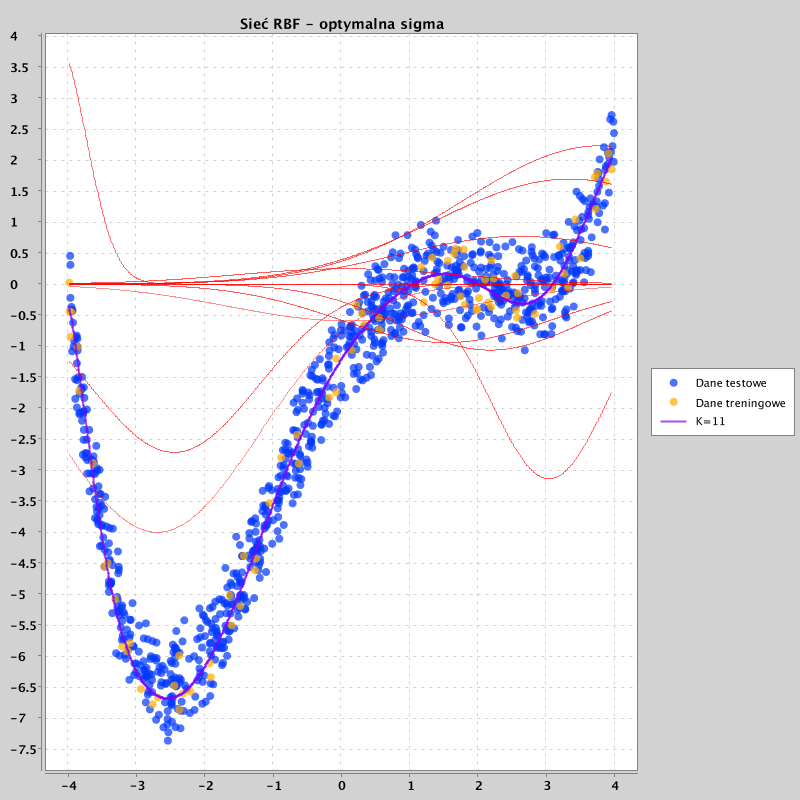
\includegraphics[width=1\linewidth]{../data/approximation3/2/derivatives/optimal.png}
    \caption{\label{fig:2optimalderivative}Optymalna sigma}
  \end{minipage}
  \begin{minipage}{0.33\textwidth}
    \centering
    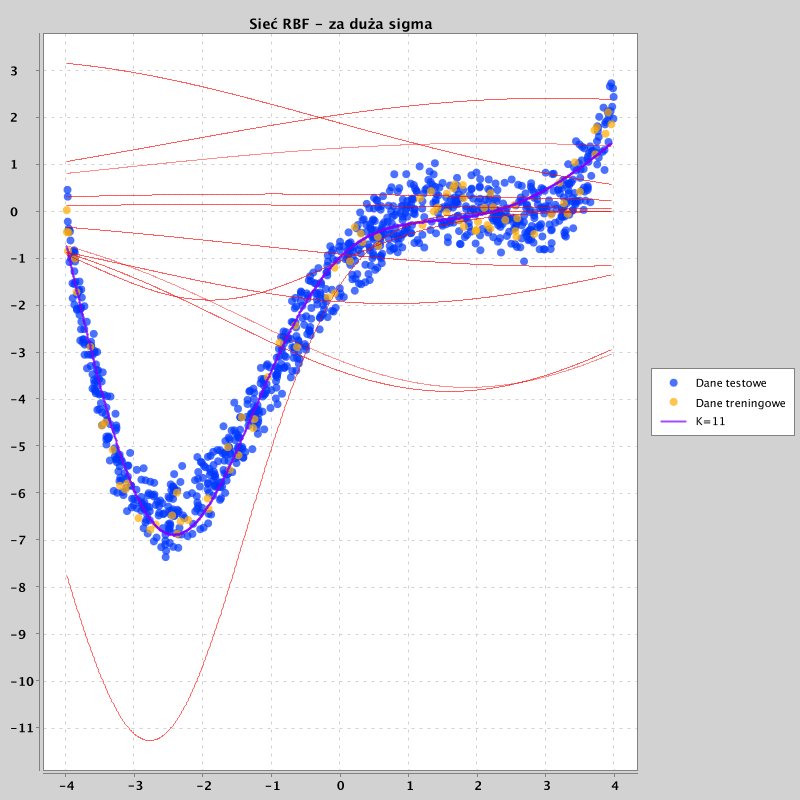
\includegraphics[width=1\linewidth]{../data/approximation3/2/derivatives/big.png}
    \caption{\label{fig:2bigderivative}Za duża sigma}
  \end{minipage}\hfill
\end{figure}

Na rysunkach \ref{fig:2smallderivative} - \ref{fig:2bigderivative} czerwonymi liniami zaznaczono funkcje realizowane przez poszczególne neurony.
W przypadku za małej sigmy można zauważyć, że sieć w celu minimalizacji błędu zmniejszyła maksymalnie współczynnik skalujący z czego wynikają zniekształcenia na wykresie \ref{fig:2smallderivative}.
Na rysunku \ref{fig:2bigderivative} widać, że tam gdzie funkcja ma prostszy kształt sigmy zostały dobrane tak, aby neurony znajdujące się w tym miejscu redukowały się wzajemnie.
W przypadku optymalnej sigmy, sieć daje bardzo dobre przybliżenie.

\subsection{Podpunkt 3}

Na rysunkach \ref{fig:41_1_4derivative} - \ref{fig:41_3_1,2,4derivative} widoczna jest zmiana skuteczności klasyfikacji.
W odróżnieniu od osobnej nauki warstw nauka przebiega znacząco szybciej. Można uznać, że sieć jest już nauczona po 500-1000 iteracji.
Poza tym, sieci są w stanie klasyfikować na poziomie 97\%, a niektóre więcej. Jest to nieznacząca różnica w porównaniu do 95\% osobnej nauki warstw.
\begin{figure}[!htb]
  \begin{minipage}{0.33\textwidth}
    \centering
    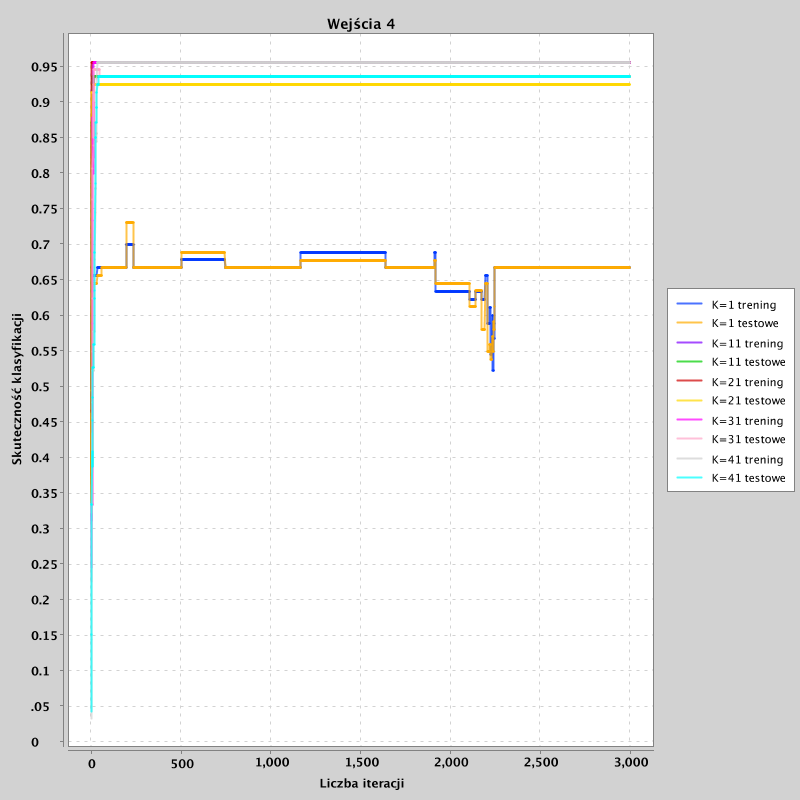
\includegraphics[width=1\linewidth]{../data/classification4/1/derivatives/1_4.png}
    \caption{\label{fig:41_1_4derivative}}
  \end{minipage}
  \begin{minipage}{0.33\textwidth}
    \centering
    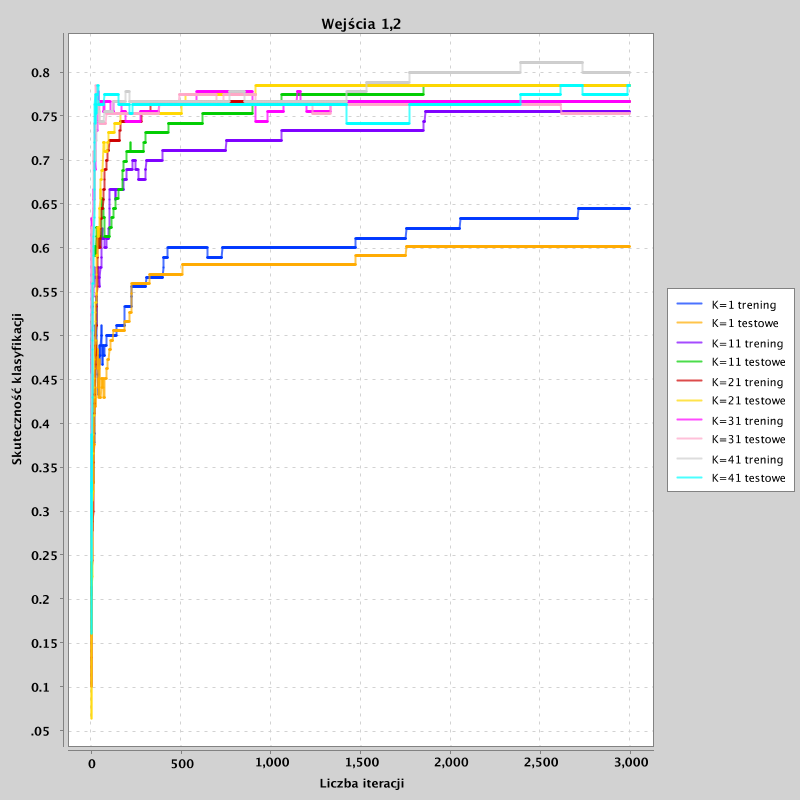
\includegraphics[width=1\linewidth]{../data/classification4/1/derivatives/2_1,2.png}
    \caption{\label{fig:41_2_1,2derivative}}
  \end{minipage}
  \begin{minipage}{0.33\textwidth}
    \centering
    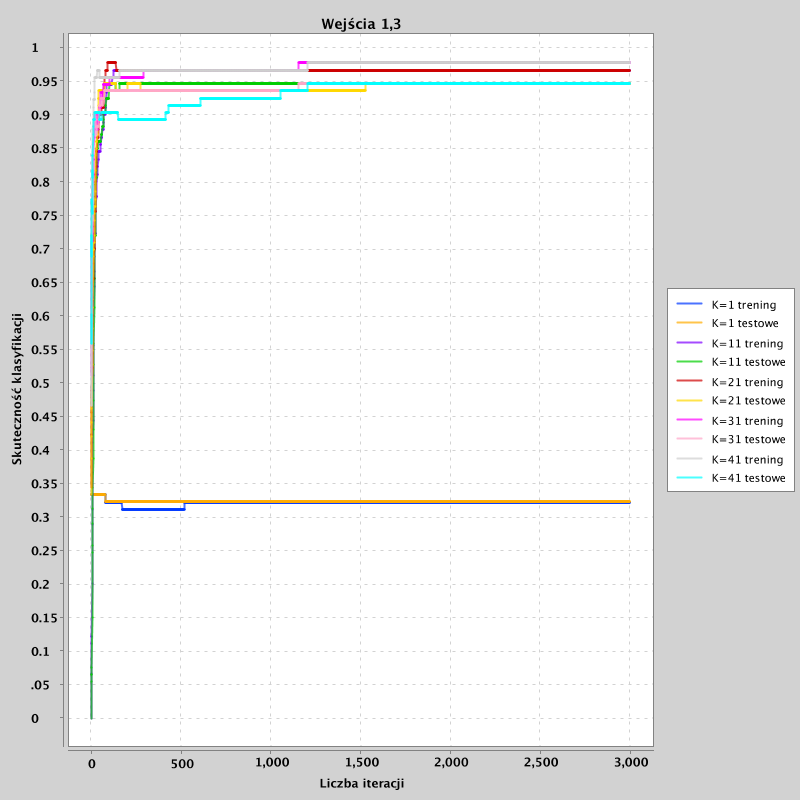
\includegraphics[width=1\linewidth]{../data/classification4/1/derivatives/2_1,3.png}
    \caption{\label{fig:41_2_1,3derivative}}
  \end{minipage}\hfill
\end{figure}
\begin{figure}[!htb]
  \begin{minipage}{0.33\textwidth}
    \centering
    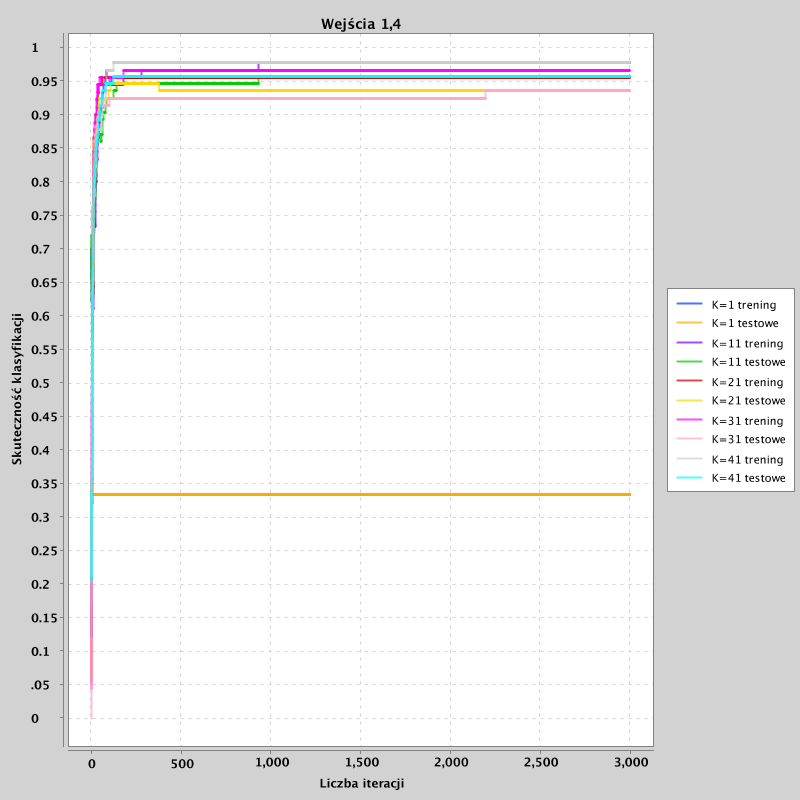
\includegraphics[width=1\linewidth]{../data/classification4/1/derivatives/2_1,4.png}
    \caption{\label{fig:41_2_1,4derivative}}
  \end{minipage}
  \begin{minipage}{0.33\textwidth}
    \centering
    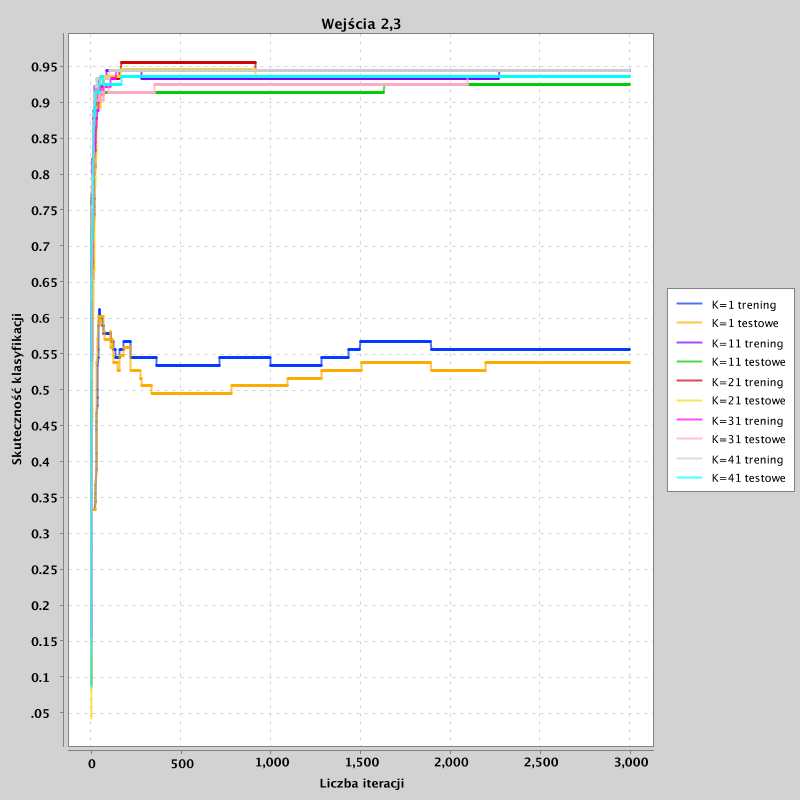
\includegraphics[width=1\linewidth]{../data/classification4/1/derivatives/2_2,3.png}
    \caption{\label{fig:41_2_2,3derivative}}
  \end{minipage}
  \begin{minipage}{0.33\textwidth}
    \centering
    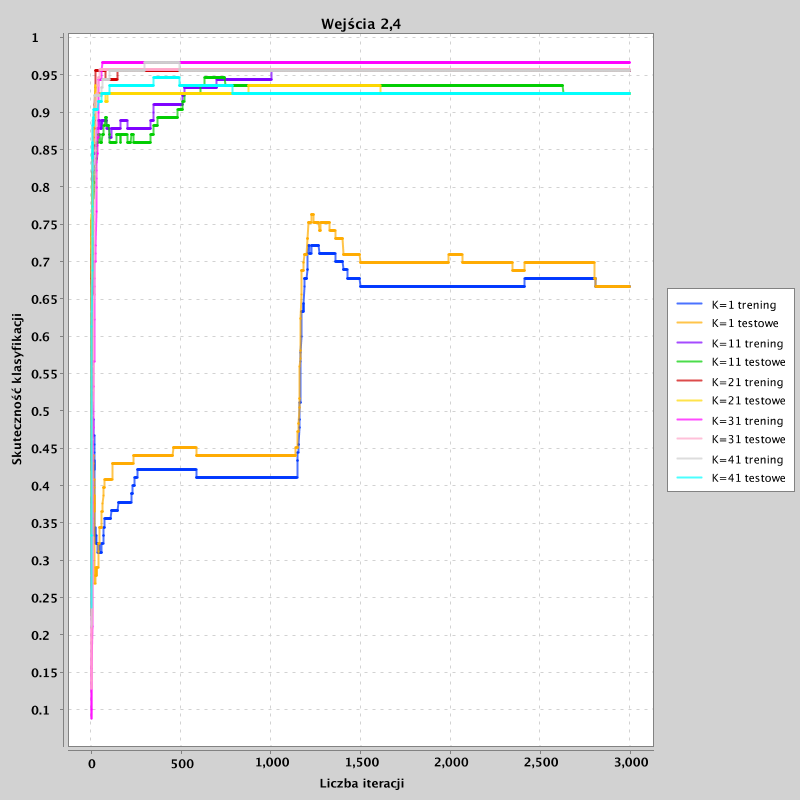
\includegraphics[width=1\linewidth]{../data/classification4/1/derivatives/2_2,4.png}
    \caption{\label{fig:41_2_2,4derivative}}
  \end{minipage}\hfill
\end{figure}
\begin{figure}[!htb]
  \begin{minipage}{0.33\textwidth}
    \centering
    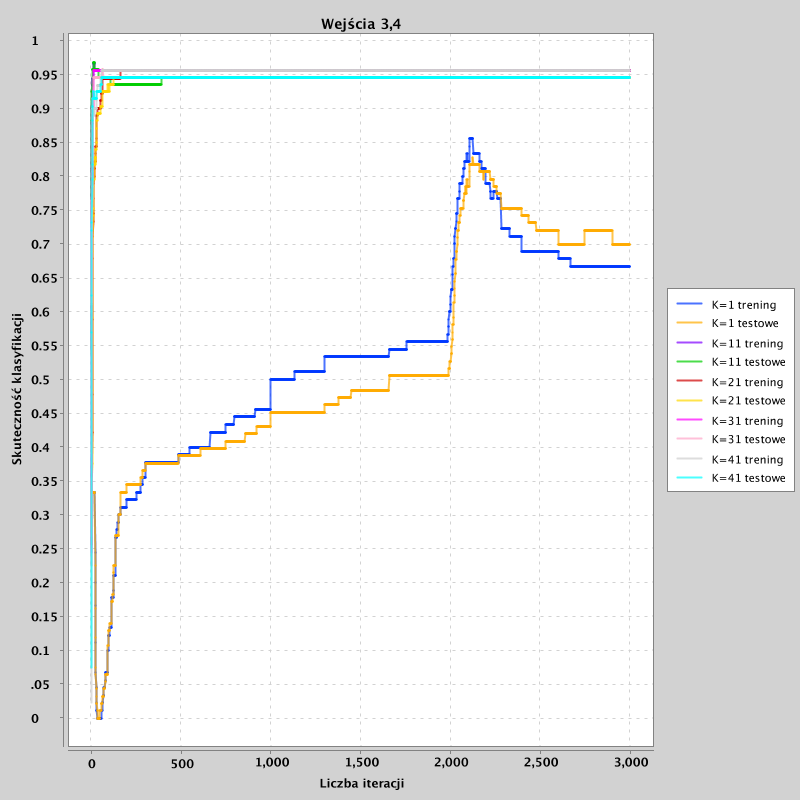
\includegraphics[width=1\linewidth]{../data/classification4/1/derivatives/2_3,4.png}
    \caption{\label{fig:41_2_3,4derivative}}
  \end{minipage}
  \begin{minipage}{0.33\textwidth}
    \centering
    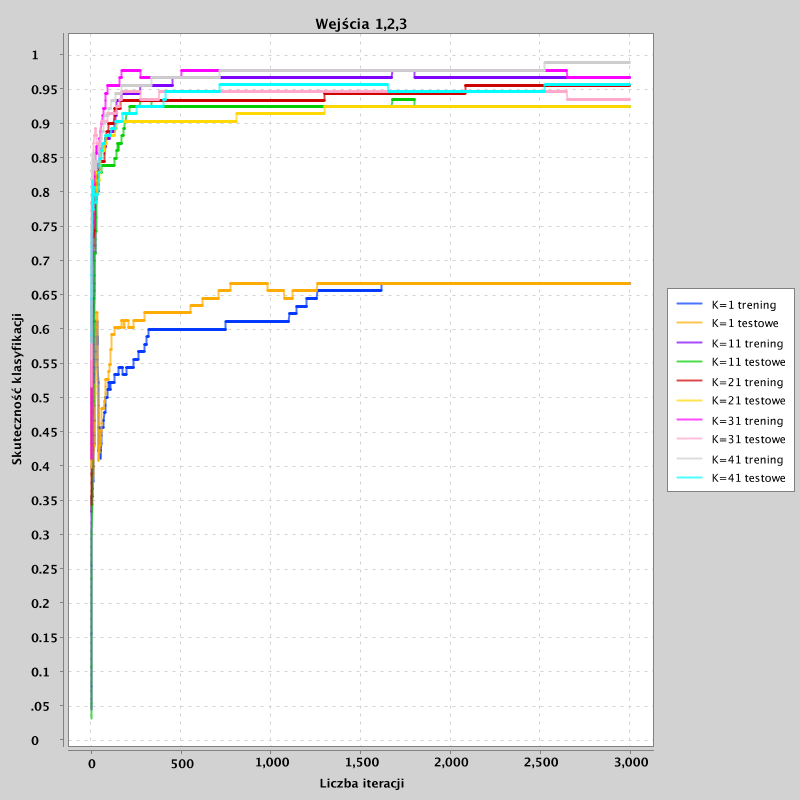
\includegraphics[width=1\linewidth]{../data/classification4/1/derivatives/3_1,2,3.png}
    \caption{\label{fig:41_3_1,2,3derivative}}
  \end{minipage}
  \begin{minipage}{0.33\textwidth}
    \centering
    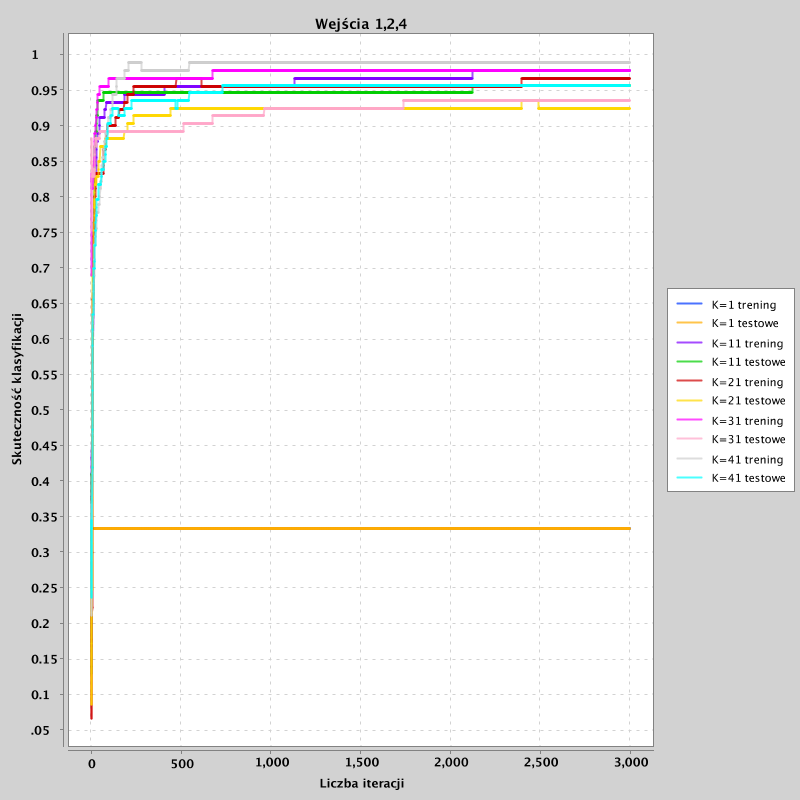
\includegraphics[width=1\linewidth]{../data/classification4/1/derivatives/3_1,2,4.png}
    \caption{\label{fig:41_3_1,2,4derivative}}
  \end{minipage}\hfill
\end{figure}
\begin{figure}[!htb]
  \begin{minipage}{0.33\textwidth}
    \centering
    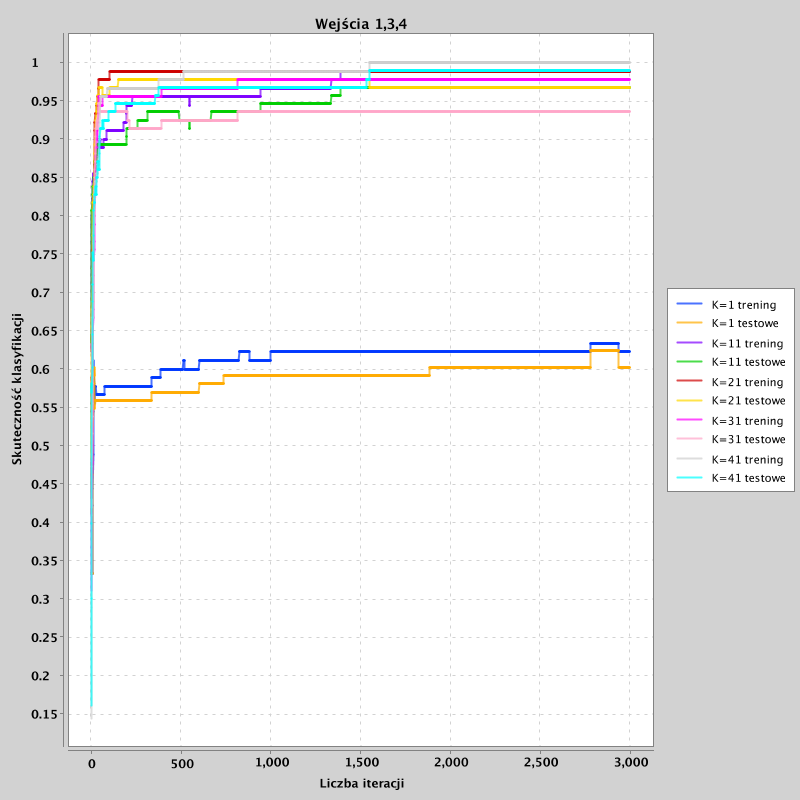
\includegraphics[width=1\linewidth]{../data/classification4/1/derivatives/3_1,3,4.png}
    \caption{\label{fig:41_3_1,3,4derivative}}
  \end{minipage}
  \begin{minipage}{0.33\textwidth}
    \centering
    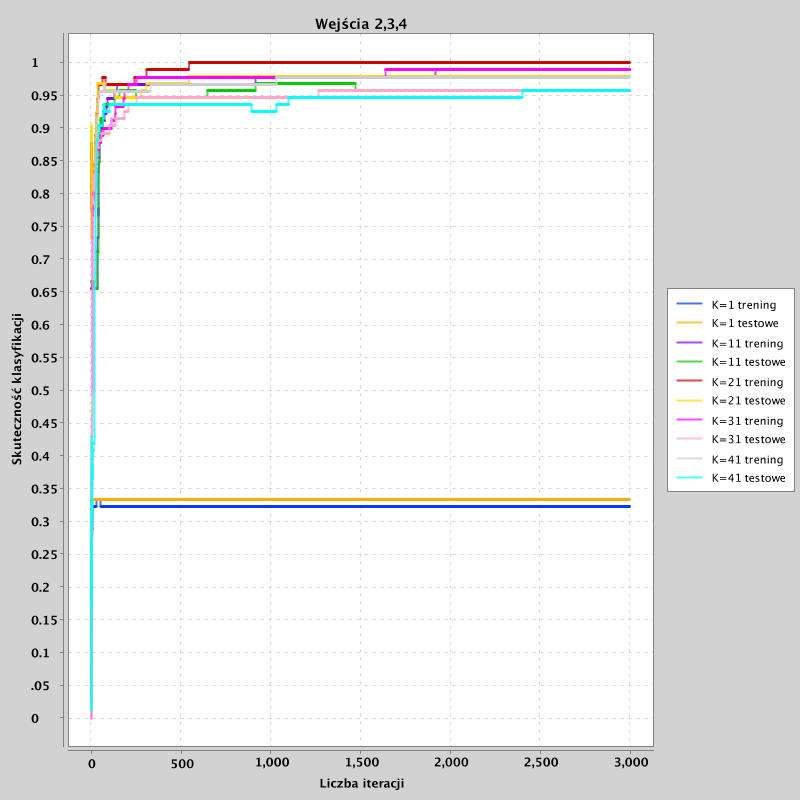
\includegraphics[width=1\linewidth]{../data/classification4/1/derivatives/3_2,3,4.png}
    \caption{\label{fig:41_3_2,3,4derivative}}
  \end{minipage}
  \begin{minipage}{0.33\textwidth}
    \centering
    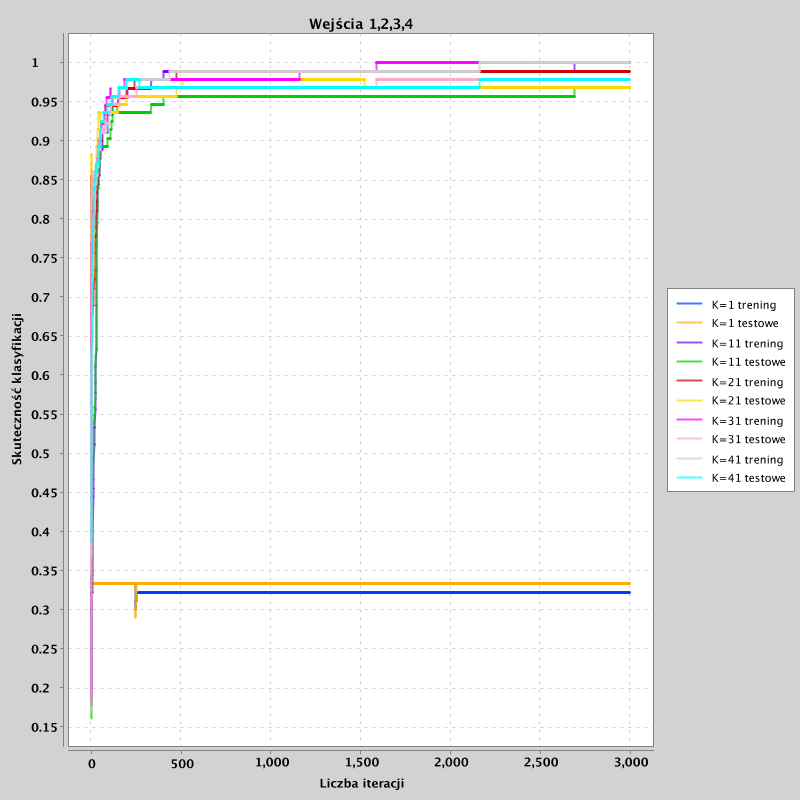
\includegraphics[width=1\linewidth]{../data/classification4/1/derivatives/4_1,2,3,4.png}
    \caption{\label{fig:41_4_1,2,3,4derivative}}
  \end{minipage}\hfill
\end{figure}


Rysunki \ref{fig:43_2_1,2derivative} - \ref{fig:43_2_3,4derivative} zostały wygenerowane dla $K=6$.
Obszary decyzyjne są bardzo zbliżone do osobnej nauki warstw, niektóre granice są bardziej dokładne.

\section{Podsumowanie}
\begin{itemize}
  \item Uczenie obydwóch warstw na raz pozwala na większy błąd w przypadku wyznaczania centrów i sigm, jednak nadal trzeba to robić aby uzyskać dobre wyniki
  \item Umożliwia szybsze nauczenie sieci, kosztem mocy obliczeniowej
  \item Ostatecznie, daje takie same albo nieznacząco lepsze wyniki niż uczenie dwóch warstw osobno
\end{itemize}

\begin{figure}[!htb]
  \begin{minipage}{0.33\textwidth}
    \centering
    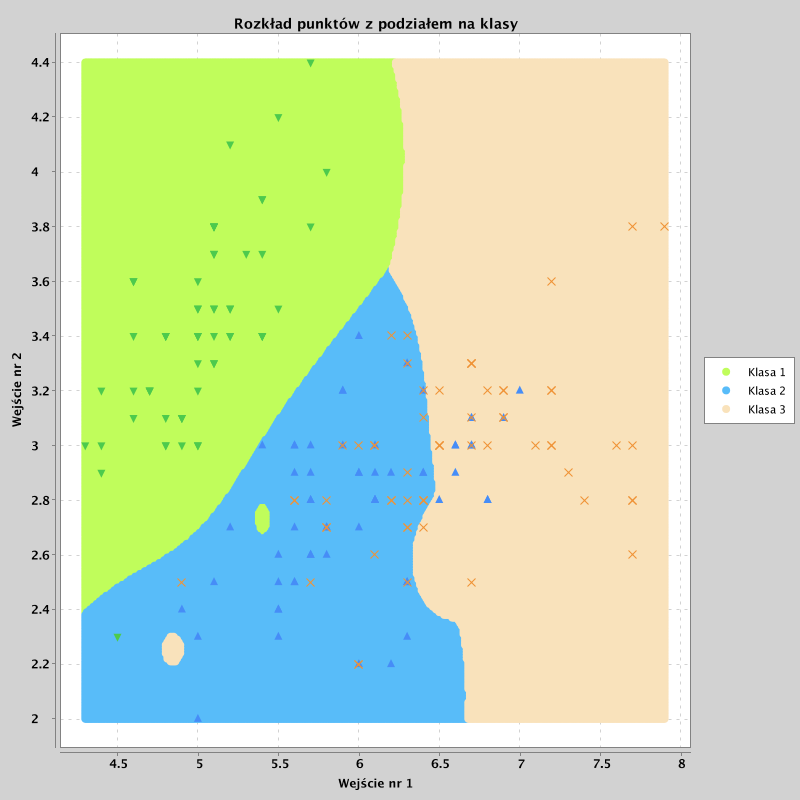
\includegraphics[width=1\linewidth]{../data/classification4/3/derivatives/2_1,2.png}
    \caption{\label{fig:43_2_1,2derivative}}
  \end{minipage}
  \begin{minipage}{0.33\textwidth}
    \centering
    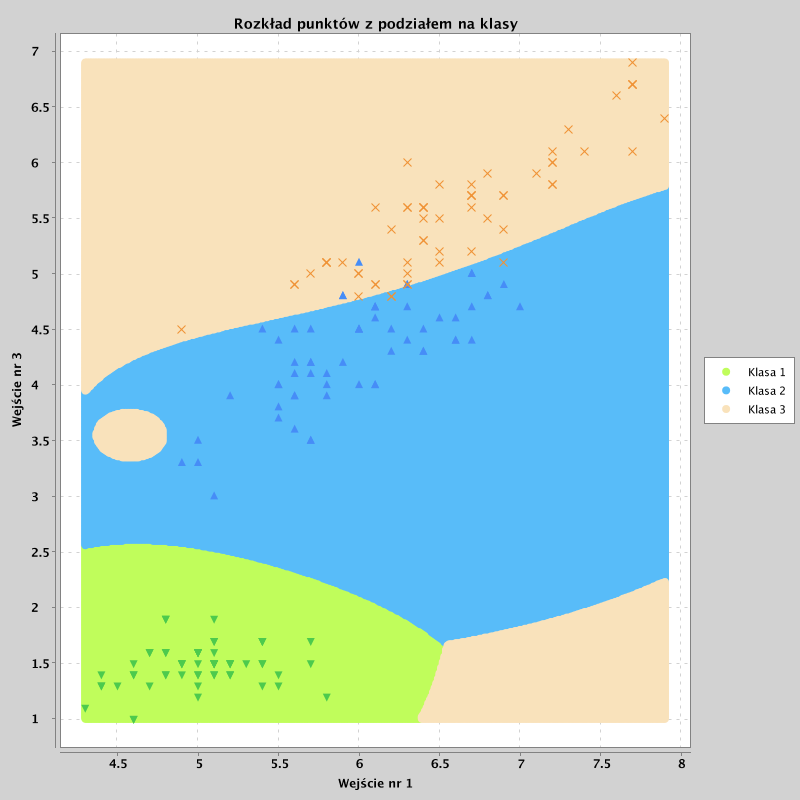
\includegraphics[width=1\linewidth]{../data/classification4/3/derivatives/2_1,3.png}
    \caption{\label{fig:43_2_1,3derivative}}
  \end{minipage}
  \begin{minipage}{0.33\textwidth}
    \centering
    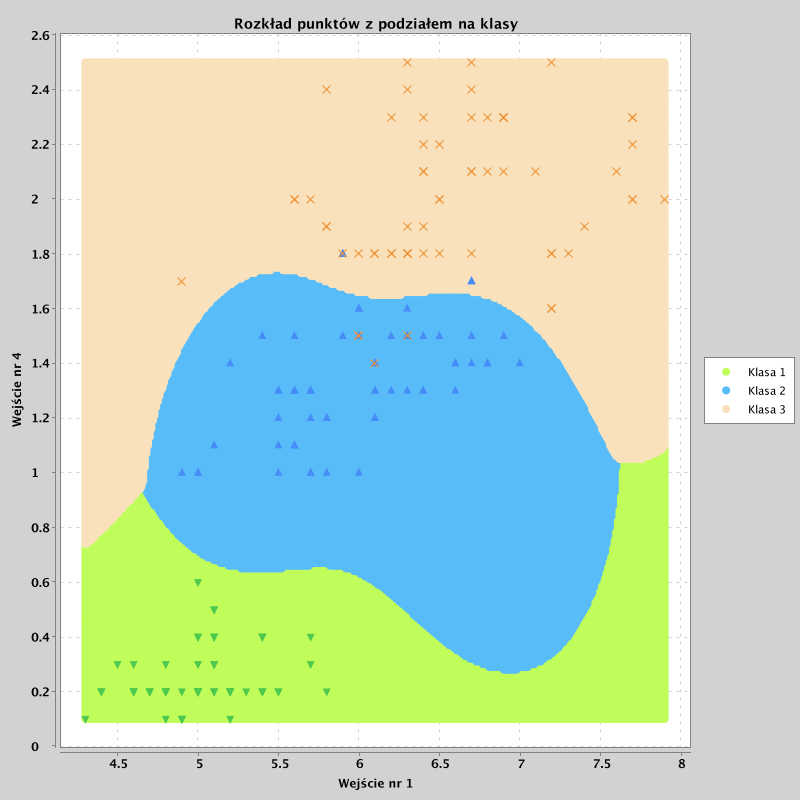
\includegraphics[width=1\linewidth]{../data/classification4/3/derivatives/2_1,4.png}
    \caption{\label{fig:43_2_1,4derivative}}
  \end{minipage}\hfill
\end{figure}
\begin{figure}[!htb]
  \begin{minipage}{0.33\textwidth}
    \centering
    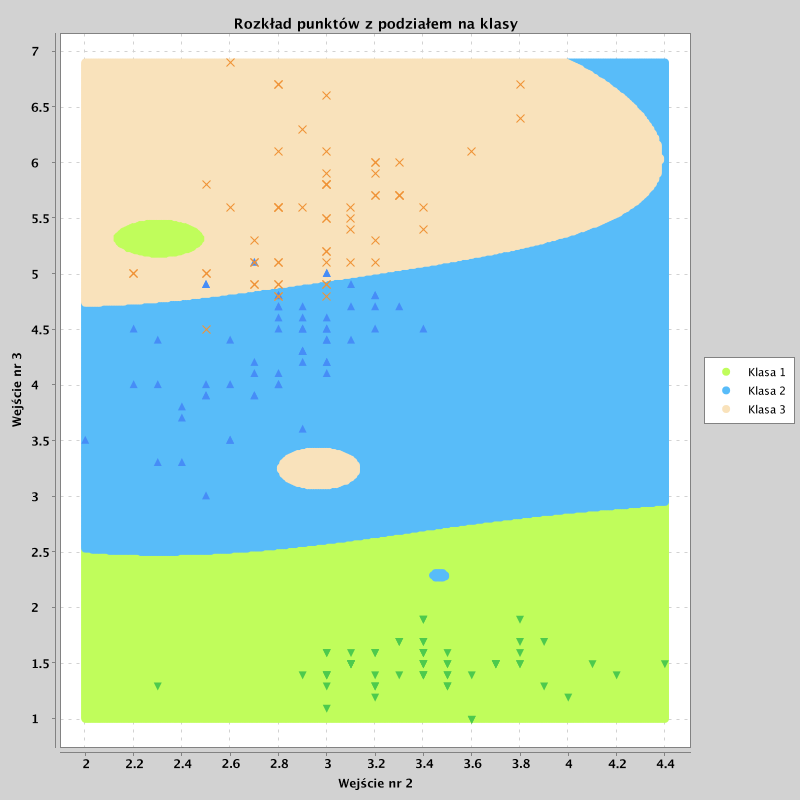
\includegraphics[width=1\linewidth]{../data/classification4/3/derivatives/2_2,3.png}
    \caption{\label{fig:43_2_2,3derivative}}
  \end{minipage}
  \begin{minipage}{0.33\textwidth}
    \centering
    \includegraphics[width=1\linewidth]{../data/classification4/3/derivatives/2_2,4.png}
    \caption{\label{fig:43_2_2,4derivative}}
  \end{minipage}
  \begin{minipage}{0.33\textwidth}
    \centering
    \includegraphics[width=1\linewidth]{../data/classification4/3/derivatives/2_3,4.png}
    \caption{\label{fig:43_2_3,4derivative}}
  \end{minipage}\hfill
\end{figure}

\end{document}